\documentclass[]{article}
\usepackage{lmodern}
\usepackage{amssymb,amsmath}
\usepackage{ifxetex,ifluatex}
\usepackage{bm}
\usepackage{soul}
\usepackage[color=yellow]{todonotes}
\usepackage{fixltx2e} % provides \textsubscript
\ifnum 0\ifxetex 1\fi\ifluatex 1\fi=0 % if pdftex
  \usepackage[T1]{fontenc}
  \usepackage[utf8]{inputenc}
\else % if luatex or xelatex
  \ifxetex
    \usepackage{mathspec}
  \else
    \usepackage{fontspec}
  \fi
  \defaultfontfeatures{Ligatures=TeX,Scale=MatchLowercase}
\fi
% use upquote if available, for straight quotes in verbatim environments
\IfFileExists{upquote.sty}{\usepackage{upquote}}{}
% use microtype if available
\IfFileExists{microtype.sty}{%
\usepackage{microtype}
\UseMicrotypeSet[protrusion]{basicmath} % disable protrusion for tt fonts
}{}
\usepackage[margin=1in]{geometry}
\usepackage{hyperref}
\hypersetup{unicode=true,
            pdftitle={8 Smoothing in the time and frequency domains},
            pdfauthor={Edward Ionides},
            pdfborder={0 0 0},
            breaklinks=true}
\urlstyle{same}  % don't use monospace font for urls
\usepackage{color}
\usepackage{fancyvrb}
\newcommand{\VerbBar}{|}
\newcommand{\VERB}{\Verb[commandchars=\\\{\}]}
\DefineVerbatimEnvironment{Highlighting}{Verbatim}{commandchars=\\\{\}}
% Add ',fontsize=\small' for more characters per line
\usepackage{framed}
\definecolor{shadecolor}{RGB}{248,248,248}
\newenvironment{Shaded}{\begin{snugshade}}{\end{snugshade}}
\newcommand{\KeywordTok}[1]{\textcolor[rgb]{0.13,0.29,0.53}{\textbf{#1}}}
\newcommand{\DataTypeTok}[1]{\textcolor[rgb]{0.13,0.29,0.53}{#1}}
\newcommand{\DecValTok}[1]{\textcolor[rgb]{0.00,0.00,0.81}{#1}}
\newcommand{\BaseNTok}[1]{\textcolor[rgb]{0.00,0.00,0.81}{#1}}
\newcommand{\FloatTok}[1]{\textcolor[rgb]{0.00,0.00,0.81}{#1}}
\newcommand{\ConstantTok}[1]{\textcolor[rgb]{0.00,0.00,0.00}{#1}}
\newcommand{\CharTok}[1]{\textcolor[rgb]{0.31,0.60,0.02}{#1}}
\newcommand{\SpecialCharTok}[1]{\textcolor[rgb]{0.00,0.00,0.00}{#1}}
\newcommand{\StringTok}[1]{\textcolor[rgb]{0.31,0.60,0.02}{#1}}
\newcommand{\VerbatimStringTok}[1]{\textcolor[rgb]{0.31,0.60,0.02}{#1}}
\newcommand{\SpecialStringTok}[1]{\textcolor[rgb]{0.31,0.60,0.02}{#1}}
\newcommand{\ImportTok}[1]{#1}
\newcommand{\CommentTok}[1]{\textcolor[rgb]{0.56,0.35,0.01}{\textit{#1}}}
\newcommand{\DocumentationTok}[1]{\textcolor[rgb]{0.56,0.35,0.01}{\textbf{\textit{#1}}}}
\newcommand{\AnnotationTok}[1]{\textcolor[rgb]{0.56,0.35,0.01}{\textbf{\textit{#1}}}}
\newcommand{\CommentVarTok}[1]{\textcolor[rgb]{0.56,0.35,0.01}{\textbf{\textit{#1}}}}
\newcommand{\OtherTok}[1]{\textcolor[rgb]{0.56,0.35,0.01}{#1}}
\newcommand{\FunctionTok}[1]{\textcolor[rgb]{0.00,0.00,0.00}{#1}}
\newcommand{\VariableTok}[1]{\textcolor[rgb]{0.00,0.00,0.00}{#1}}
\newcommand{\ControlFlowTok}[1]{\textcolor[rgb]{0.13,0.29,0.53}{\textbf{#1}}}
\newcommand{\OperatorTok}[1]{\textcolor[rgb]{0.81,0.36,0.00}{\textbf{#1}}}
\newcommand{\BuiltInTok}[1]{#1}
\newcommand{\ExtensionTok}[1]{#1}
\newcommand{\PreprocessorTok}[1]{\textcolor[rgb]{0.56,0.35,0.01}{\textit{#1}}}
\newcommand{\AttributeTok}[1]{\textcolor[rgb]{0.77,0.63,0.00}{#1}}
\newcommand{\RegionMarkerTok}[1]{#1}
\newcommand{\InformationTok}[1]{\textcolor[rgb]{0.56,0.35,0.01}{\textbf{\textit{#1}}}}
\newcommand{\WarningTok}[1]{\textcolor[rgb]{0.56,0.35,0.01}{\textbf{\textit{#1}}}}
\newcommand{\AlertTok}[1]{\textcolor[rgb]{0.94,0.16,0.16}{#1}}
\newcommand{\ErrorTok}[1]{\textcolor[rgb]{0.64,0.00,0.00}{\textbf{#1}}}
\newcommand{\NormalTok}[1]{#1}
\usepackage{longtable,booktabs}
\usepackage{graphicx,grffile}
\makeatletter
\def\maxwidth{\ifdim\Gin@nat@width>\linewidth\linewidth\else\Gin@nat@width\fi}
\def\maxheight{\ifdim\Gin@nat@height>\textheight\textheight\else\Gin@nat@height\fi}
\makeatother
% Scale images if necessary, so that they will not overflow the page
% margins by default, and it is still possible to overwrite the defaults
% using explicit options in \includegraphics[width, height, ...]{}
\setkeys{Gin}{width=\maxwidth,height=\maxheight,keepaspectratio}
\IfFileExists{parskip.sty}{%
\usepackage{parskip}
}{% else
\setlength{\parindent}{0pt}
\setlength{\parskip}{6pt plus 2pt minus 1pt}
}
\setlength{\emergencystretch}{3em}  % prevent overfull lines
\providecommand{\tightlist}{%
  \setlength{\itemsep}{0pt}\setlength{\parskip}{0pt}}
%\setcounter{secnumdepth}{0}
\setcounter{section}{8}
% Redefines (sub)paragraphs to behave more like sections
\ifx\paragraph\undefined\else
\let\oldparagraph\paragraph
\renewcommand{\paragraph}[1]{\oldparagraph{#1}\mbox{}}
\fi
\ifx\subparagraph\undefined\else
\let\oldsubparagraph\subparagraph
\renewcommand{\subparagraph}[1]{\oldsubparagraph{#1}\mbox{}}
\fi

%%% Use protect on footnotes to avoid problems with footnotes in titles
\let\rmarkdownfootnote\footnote%
\def\footnote{\protect\rmarkdownfootnote}

%%% Change title format to be more compact
\usepackage{titling}

% Create subtitle command for use in maketitle
\newcommand{\subtitle}[1]{
  \posttitle{
    \begin{center}\large#1\end{center}
    }
}

\setlength{\droptitle}{-2em}
  \title{8. Smoothing in the time and frequency domains}
  \pretitle{\vspace{\droptitle}\centering\huge}
  \posttitle{\par}
  \author{Edward Ionides}
  \preauthor{\centering\large\emph}
  \postauthor{\par}
  \predate{\centering\large\emph}
  \postdate{\par}
  \date{2/7/2018}


\begin{document}
\maketitle

{
\setcounter{tocdepth}{2}
\tableofcontents
}
\newcommand\prob{\mathbb{P}}
\newcommand\E{\mathbb{E}}
\newcommand\var{\mathrm{Var}}
\newcommand\cov{\mathrm{Cov}}
\newcommand\loglik{\ell}
\newcommand\R{\mathbb{R}}
\newcommand\data[1]{#1^*}
\newcommand\params{\, ; \,}
\newcommand\transpose{\scriptsize{T}}
\newcommand\eqspace{\quad\quad\quad}
\newcommand\lik{\mathscr{L}}
\newcommand\profileloglik[1]{\ell^\mathrm{profile}_#1}
\newcommand\ar{\phi}
\newcommand\ma{\psi}
\newcommand\AR{\Phi}
\newcommand\MA{\Psi}
\newcommand\ev{u}





\begin{center}\rule{0.5\linewidth}{\linethickness}\end{center}

\begin{center}\rule{0.5\linewidth}{\linethickness}\end{center}

Objectives

\begin{itemize}
\item
  \hl{Estimating a nonparametric trend from a time series is known as
  smoothing}. We will review some standard smoothing methods.
\item
  We can also smooth the periodogram to estimate a spectral density.
\item
  Many smoothers can be represented as linear filters. We will see that
  the statistical properties of linear filters for dependent
  (time-domain) stationary models can be conveniently studied in the
  frequency domain.
\end{itemize}

\begin{center}\rule{0.5\linewidth}{\linethickness}\end{center}

\begin{center}\rule{0.5\linewidth}{\linethickness}\end{center}

\subsection{A motivating example}\label{a-motivating-example}

\begin{itemize}
\item
  The economy fluctuates between periods of rapid expansion and periods
  of slower growth or contraction.
\item
  High unemployment is one of the most visible signs of a dysfunctional
  economy, in which labor is under-utilized, leading to hardships for
  many individuals and communities.
\item
  Economists, politicians, businesspeople and the general public
  therefore have an interest in understanding fluctuations in
  unemployment.
\item
  Economists try to distinguish between fundamental structural changes
  in the economy and the shorter-term cyclical booms and busts that
  appear to be a natural part of capitalist business activity.
\item
  \href{http://data.bls.gov/timeseries/LNU04000000}{Monthly unemployment
  figures} for the USA are published by the Bureau of Labor Statistics.
  Measuring unemployment has subtleties, which should be acknowledged
  but are not the focus of our current exploration.
\end{itemize}

\begin{Shaded}
\begin{Highlighting}[]
\KeywordTok{system}\NormalTok{(}\StringTok{"head unadjusted_unemployment.csv"}\NormalTok{,}\DataTypeTok{intern=}\OtherTok{TRUE}\NormalTok{)}
\end{Highlighting}
\end{Shaded}

\begin{verbatim}
##  [1] "# Data extracted on: February 4, 2016 (10:06:56 AM)"        
##  [2] "# from http://data.bls.gov/timeseries/LNU04000000"          
##  [3] "# Labor Force Statistics from the Current Population Survey"
##  [4] "# Not Seasonally Adjusted"                                  
##  [5] "# Series title:        (Unadj) Unemployment Rate"           
##  [6] "# Labor force status:  Unemployment rate"                   
##  [7] "# Type of data:        Percent or rate"                     
##  [8] "# Age:                 16 years and over"                   
##  [9] "Year,Jan,Feb,Mar,Apr,May,Jun,Jul,Aug,Sep,Oct,Nov,Dec"       
## [10] "1948,4.0,4.7,4.5,4.0,3.4,3.9,3.9,3.6,3.4,2.9,3.3,3.6"
\end{verbatim}

\begin{Shaded}
\begin{Highlighting}[]
\NormalTok{U1 <-}\StringTok{ }\KeywordTok{read.table}\NormalTok{(}\DataTypeTok{file=}\StringTok{"unadjusted_unemployment.csv"}\NormalTok{,}\DataTypeTok{sep=}\StringTok{","}\NormalTok{,}\DataTypeTok{header=}\OtherTok{TRUE}\NormalTok{)}
\KeywordTok{head}\NormalTok{(U1)}
\end{Highlighting}
\end{Shaded}

\begin{verbatim}
##   Year Jan Feb Mar Apr May Jun Jul Aug Sep Oct Nov Dec
## 1 1948 4.0 4.7 4.5 4.0 3.4 3.9 3.9 3.6 3.4 2.9 3.3 3.6
## 2 1949 5.0 5.8 5.6 5.4 5.7 6.4 7.0 6.3 5.9 6.1 5.7 6.0
## 3 1950 7.6 7.9 7.1 6.0 5.3 5.6 5.3 4.1 4.0 3.3 3.8 3.9
## 4 1951 4.4 4.2 3.8 3.2 2.9 3.4 3.3 2.9 3.0 2.8 3.2 2.9
## 5 1952 3.7 3.8 3.3 3.0 2.9 3.2 3.3 3.1 2.7 2.4 2.5 2.5
## 6 1953 3.4 3.2 2.9 2.8 2.5 2.7 2.7 2.4 2.6 2.5 3.2 4.2
\end{verbatim}

\begin{itemize}
\tightlist
\item
  The data are in a table, and we want a time series. Here's one way to
  do that.
\end{itemize}

\begin{Shaded}
\begin{Highlighting}[]
\NormalTok{u1 <-}\StringTok{ }\KeywordTok{t}\NormalTok{(}\KeywordTok{as.matrix}\NormalTok{(U1[}\DecValTok{2}\OperatorTok{:}\DecValTok{13}\NormalTok{]))}
\KeywordTok{dim}\NormalTok{(u1) <-}\StringTok{ }\OtherTok{NULL}
\NormalTok{date <-}\StringTok{ }\KeywordTok{seq}\NormalTok{(}\DataTypeTok{from=}\DecValTok{1948}\NormalTok{,}\DataTypeTok{length=}\KeywordTok{length}\NormalTok{(u1),}\DataTypeTok{by=}\DecValTok{1}\OperatorTok{/}\DecValTok{12}\NormalTok{)}
\KeywordTok{plot}\NormalTok{(date,u1,}\DataTypeTok{type=}\StringTok{"l"}\NormalTok{,}\DataTypeTok{ylab=}\StringTok{"Percent unemployment (unadjusted)"}\NormalTok{)}
\end{Highlighting}
\end{Shaded}

\begin{center}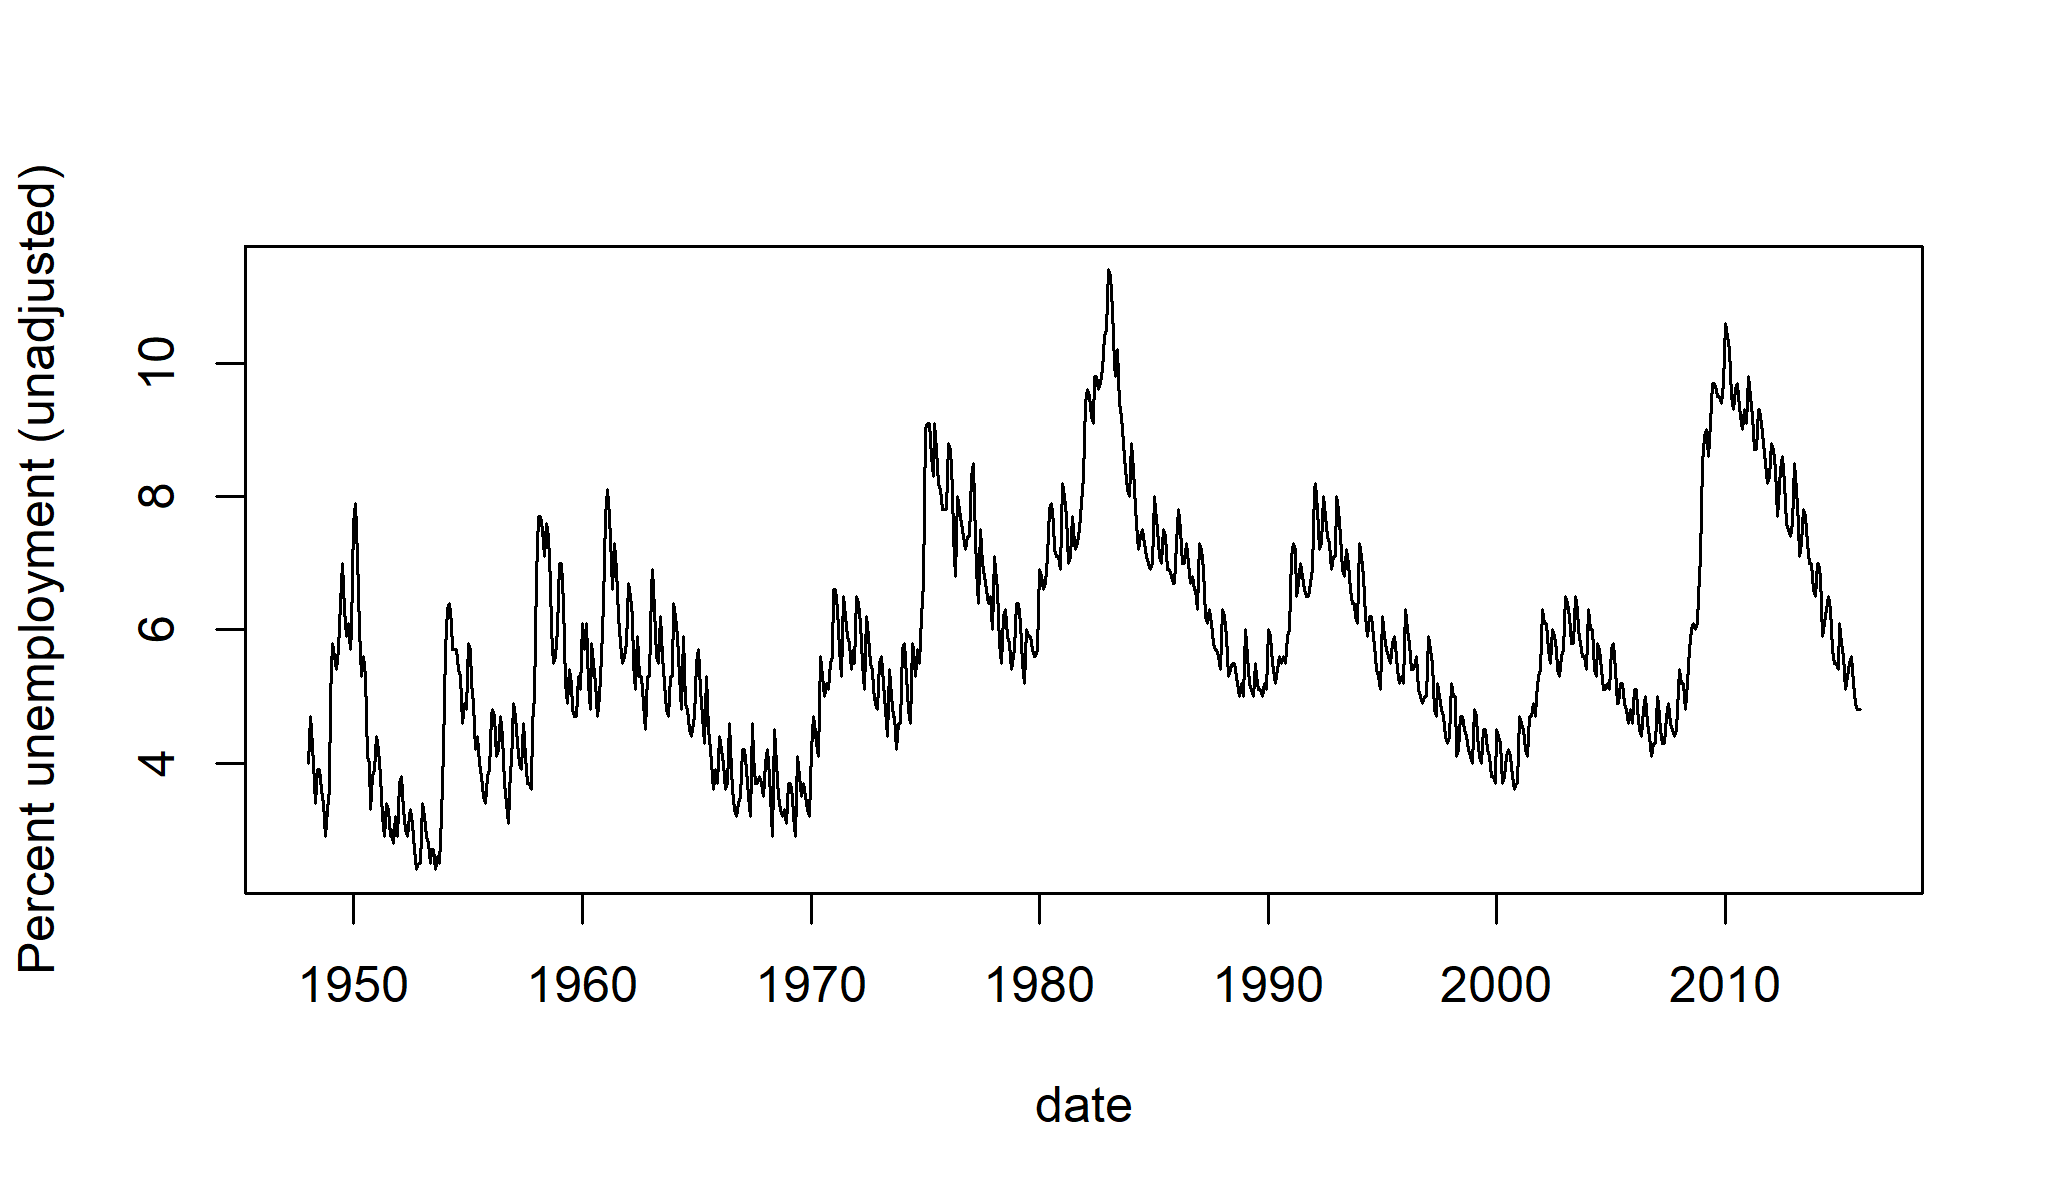
\includegraphics{figure/intro-reshape-1} \end{center}

\begin{itemize}
\item
  We see seasonal variation, and perhaps we see business cycles on top
  of a slower trend.
\item
  The seasonal variation looks like an additive effect, say an annual
  fluctation with amplitude around 1 percentage point. For many
  purposes, we may prefer to look at a measure of
  \href{http://data.bls.gov/timeseries/LNS14000000}{monthly seasonally
  adjusted unemployment}, which the Bureau of Labor Statistics also
  provides.
\end{itemize}

\begin{Shaded}
\begin{Highlighting}[]
\NormalTok{U2 <-}\StringTok{ }\KeywordTok{read.table}\NormalTok{(}\DataTypeTok{file=}\StringTok{"adjusted_unemployment.csv"}\NormalTok{,}\DataTypeTok{sep=}\StringTok{","}\NormalTok{,}\DataTypeTok{header=}\OtherTok{TRUE}\NormalTok{)}
\NormalTok{u2 <-}\StringTok{ }\KeywordTok{t}\NormalTok{(}\KeywordTok{as.matrix}\NormalTok{(U2[}\DecValTok{2}\OperatorTok{:}\DecValTok{13}\NormalTok{]))}
\KeywordTok{dim}\NormalTok{(u2) <-}\StringTok{ }\OtherTok{NULL}
\KeywordTok{plot}\NormalTok{(date,u1,}\DataTypeTok{type=}\StringTok{"l"}\NormalTok{,}\DataTypeTok{ylab=}\StringTok{"percent"}\NormalTok{,}\DataTypeTok{col=}\StringTok{"black"}\NormalTok{)}
\KeywordTok{lines}\NormalTok{(date,u2,}\DataTypeTok{type=}\StringTok{"l"}\NormalTok{,}\DataTypeTok{col=}\StringTok{"red"}\NormalTok{)}
\KeywordTok{title}\NormalTok{(}\StringTok{"Unemployment. Raw (black) and seasonally adjusted (red)"}\NormalTok{)}
\end{Highlighting}
\end{Shaded}

\begin{center}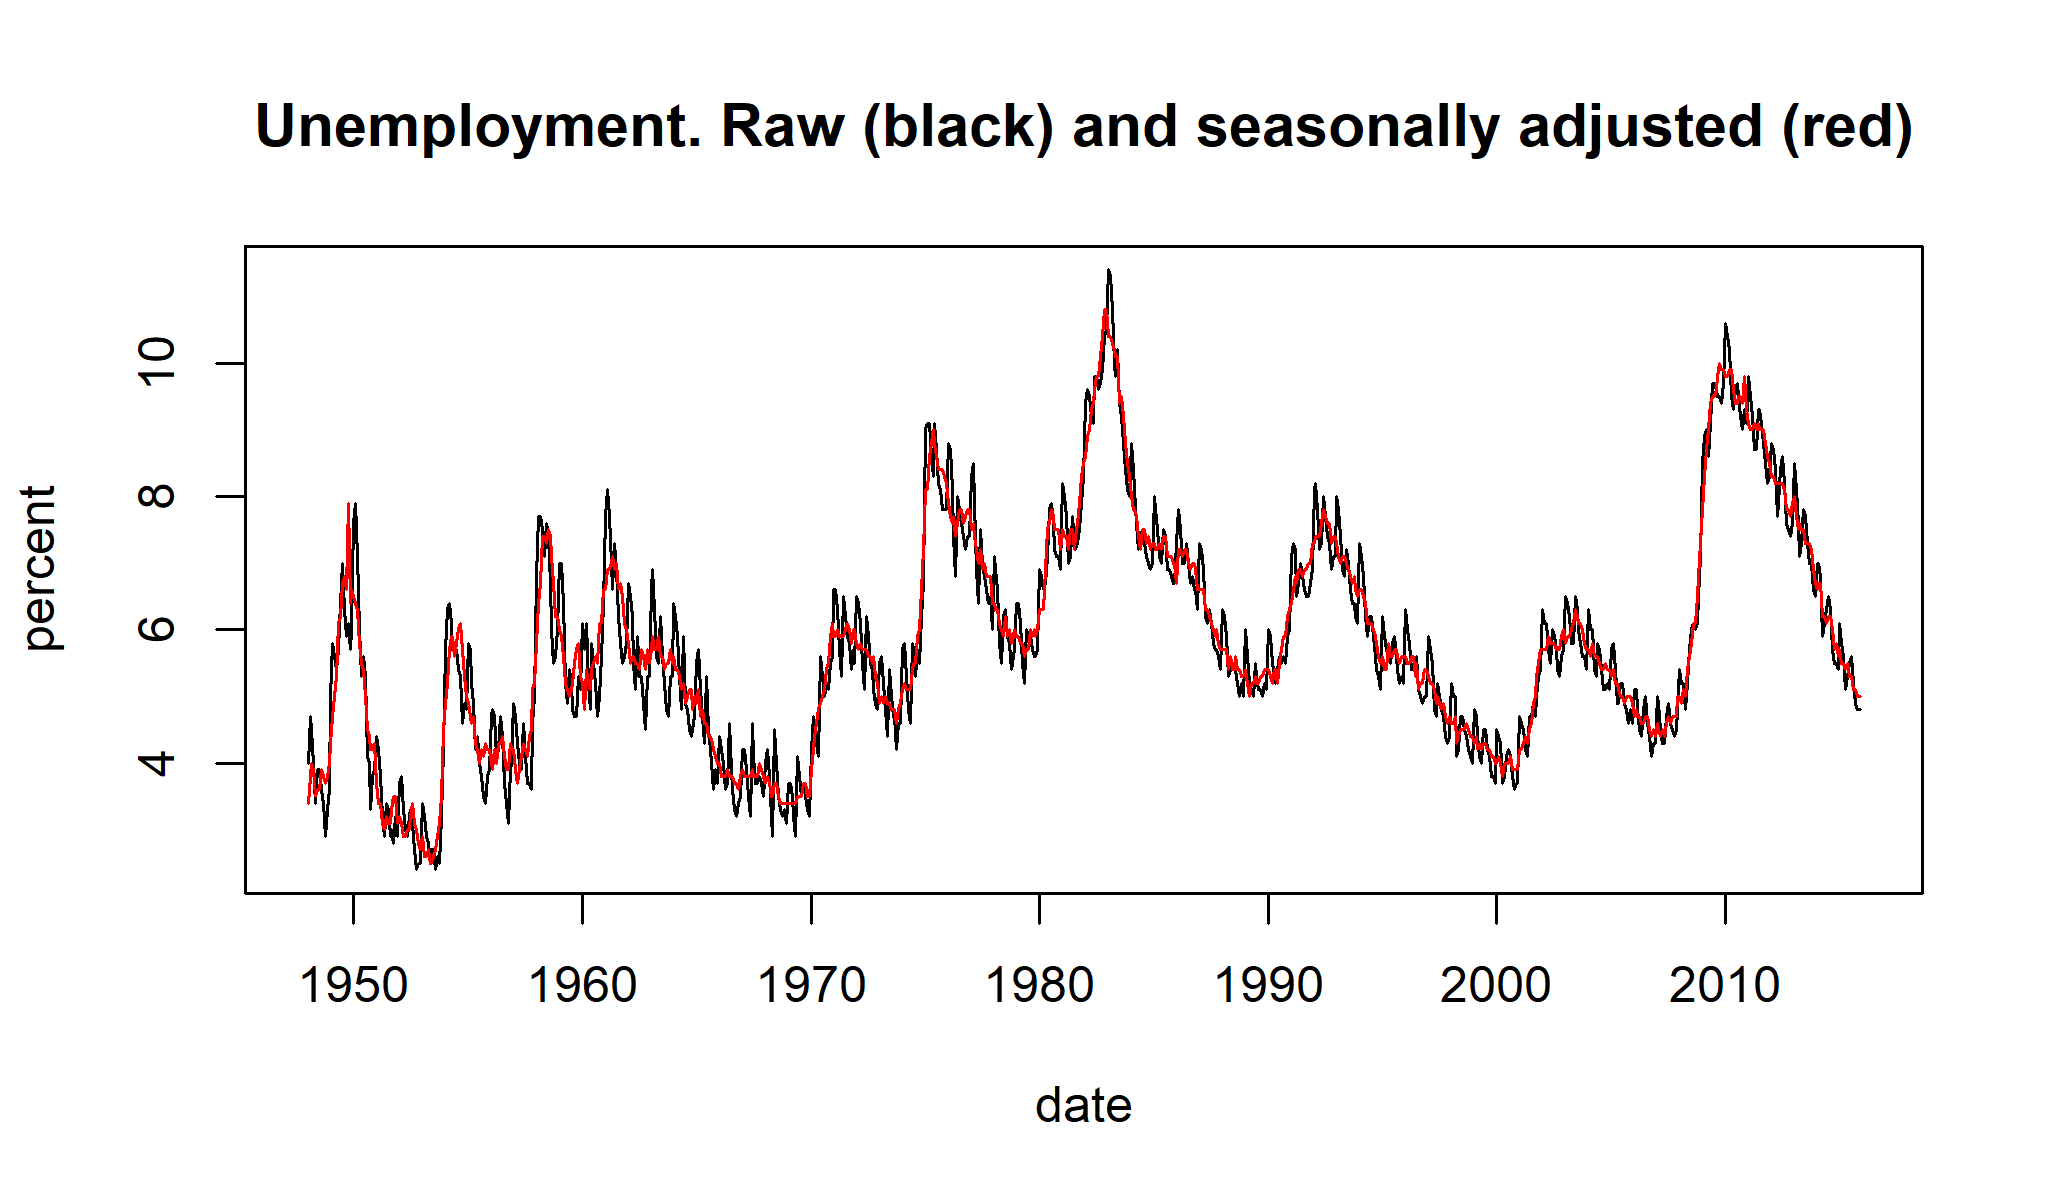
\includegraphics{figure/intro-data_adj-1} \end{center}

\begin{itemize}
\item
  As statisticians, we may be curious about how the Bureau of Labor
  Statistics adjusts the data, and whether this might introduce any
  artifacts that a careful statistician should be aware of.
\item
  Let's look at what the adjustment does to the smoothed periodogram.
\item
  To help R figure out units for plotting the spectrum, we're going to
  put our time series in the \texttt{ts} class.
\end{itemize}

\begin{Shaded}
\begin{Highlighting}[]
\NormalTok{u1_ts <-}\StringTok{ }\KeywordTok{ts}\NormalTok{(u1,}\DataTypeTok{start=}\DecValTok{1948}\NormalTok{,}\DataTypeTok{frequency=}\DecValTok{12}\NormalTok{)}
\NormalTok{u2_ts <-}\StringTok{ }\KeywordTok{ts}\NormalTok{(u2,}\DataTypeTok{start=}\DecValTok{1948}\NormalTok{,}\DataTypeTok{frequency=}\DecValTok{12}\NormalTok{)}
\KeywordTok{spectrum}\NormalTok{(}\KeywordTok{ts.union}\NormalTok{(u1_ts,u2_ts),}\DataTypeTok{spans=}\KeywordTok{c}\NormalTok{(}\DecValTok{3}\NormalTok{,}\DecValTok{5}\NormalTok{,}\DecValTok{3}\NormalTok{),}\DataTypeTok{main=}\StringTok{"Unemployment. Raw (black) and seasonally adjusted (red)"}\NormalTok{)}
\end{Highlighting}
\end{Shaded}

\begin{center}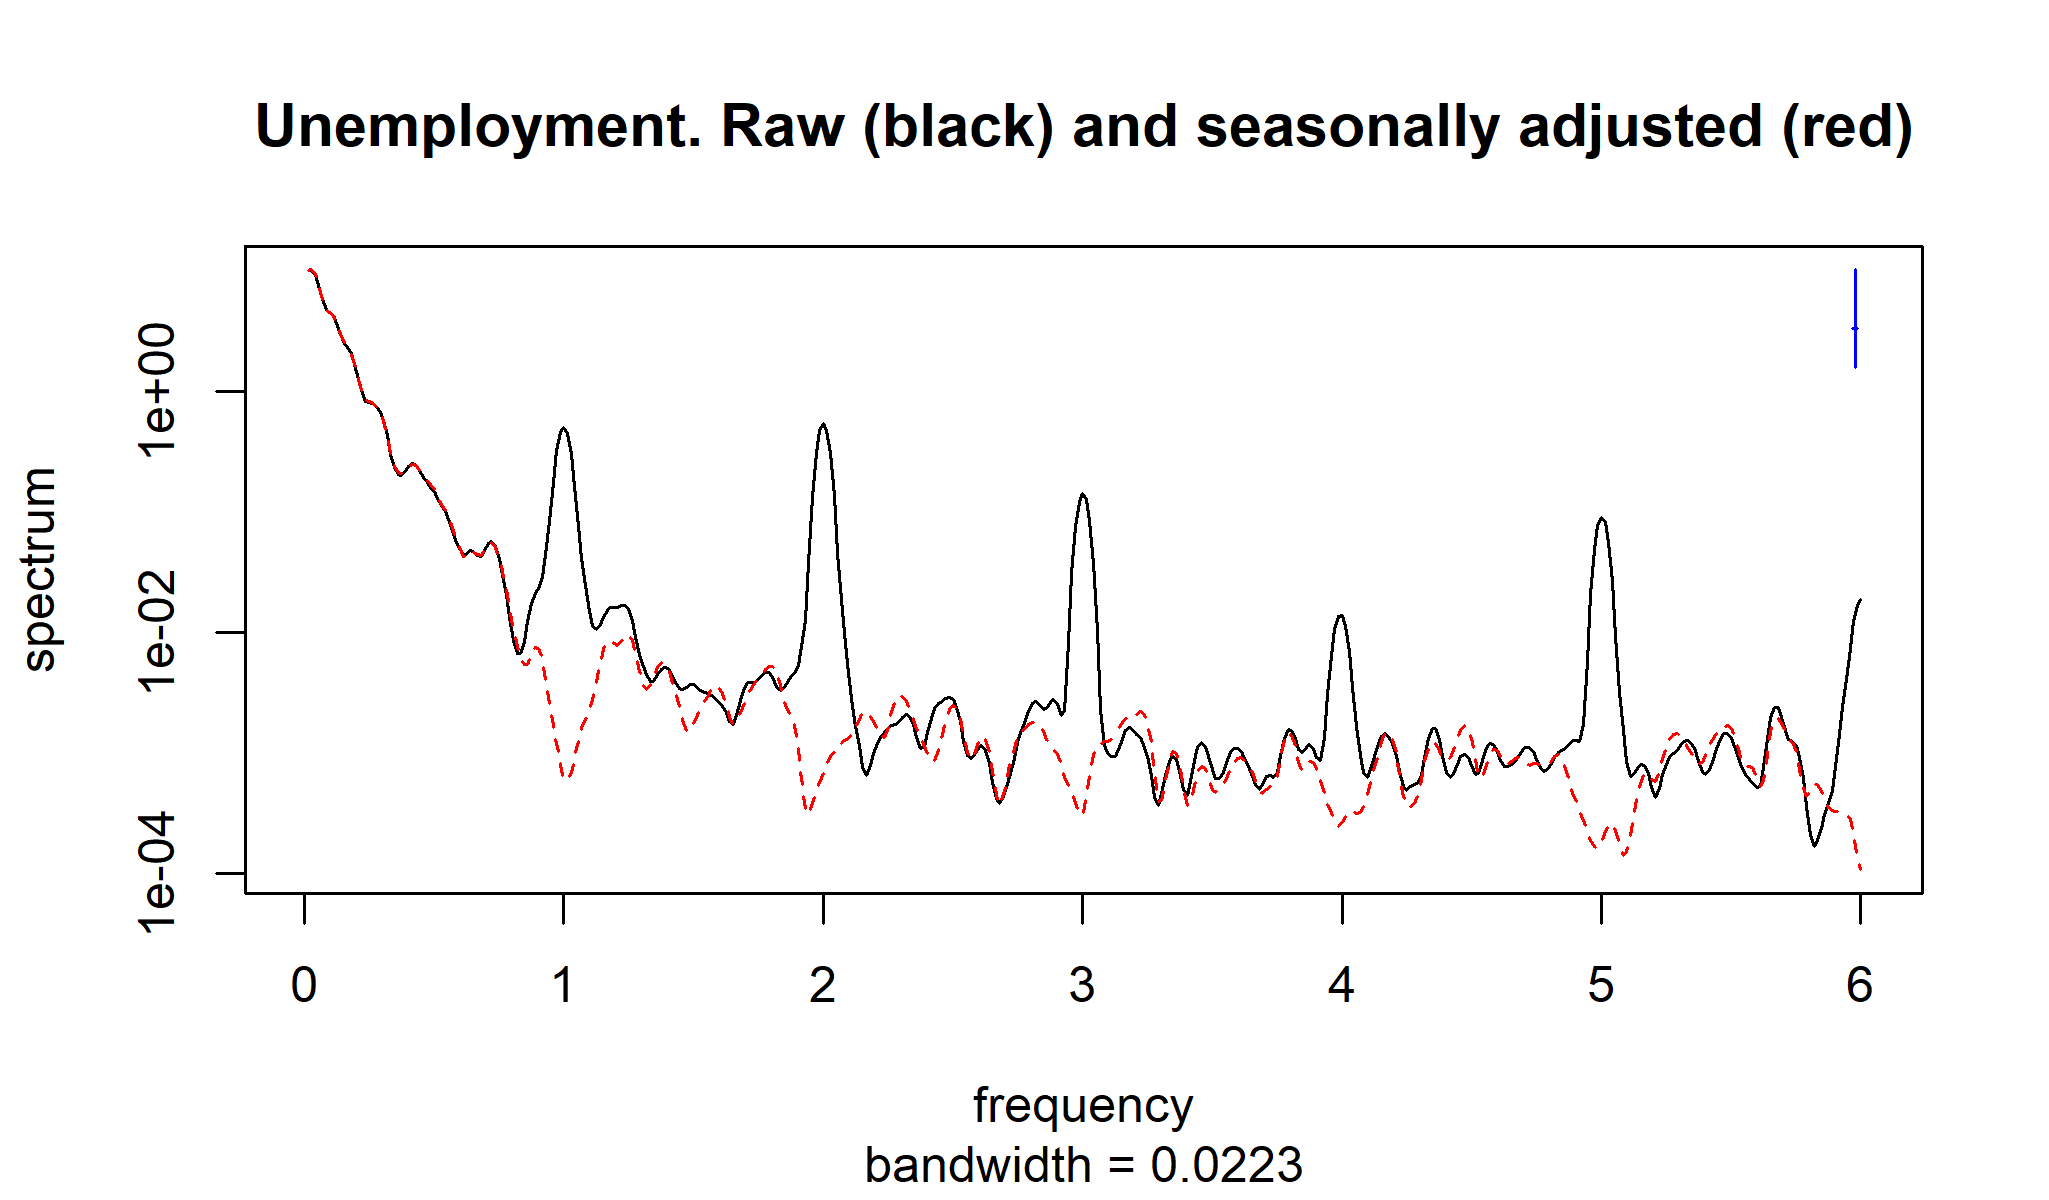
\includegraphics{figure/intro-adjustment_spectrum-1} \end{center}

\todo[inline]{Why peaks at 2, 3, 4, 5, 6 cycles per year? A peak at only 1 cycle per year is sinusoidal seasonality. The 2-cycle might be the idea that there's less unemployment during summer and winter (Christmas time).}

\begin{center}\rule{0.5\linewidth}{\linethickness}\end{center}

\begin{center}\rule{0.5\linewidth}{\linethickness}\end{center}

\subsubsection{Question: What are the x-axis
units?}\label{question-what-are-the-x-axis-units}

\todo[inline]{Cycles-per-year (rather than cycles-per-month). This more natural unit of frequency came about from the \textit{ts} function in \textit{R}, and setting the frequency to 12.}

\begin{center}\rule{0.5\linewidth}{\linethickness}\end{center}

\begin{center}\rule{0.5\linewidth}{\linethickness}\end{center}

\subsubsection{Question: Comment on what you learn from comparing these
smoothed
periodograms.}\label{question-comment-on-what-you-learn-from-comparing-these-smoothed-periodograms.}

\begin{center}\rule{0.5\linewidth}{\linethickness}\end{center}

\begin{center}\rule{0.5\linewidth}{\linethickness}\end{center}

\begin{itemize}
\tightlist
\item
  Note: the \texttt{ts} class can also be useful for helping R choose
  other plotting options in a way appriate for time series. For example,
\end{itemize}

\begin{Shaded}
\begin{Highlighting}[]
\KeywordTok{plot}\NormalTok{(u1_ts)}
\end{Highlighting}
\end{Shaded}

\begin{center}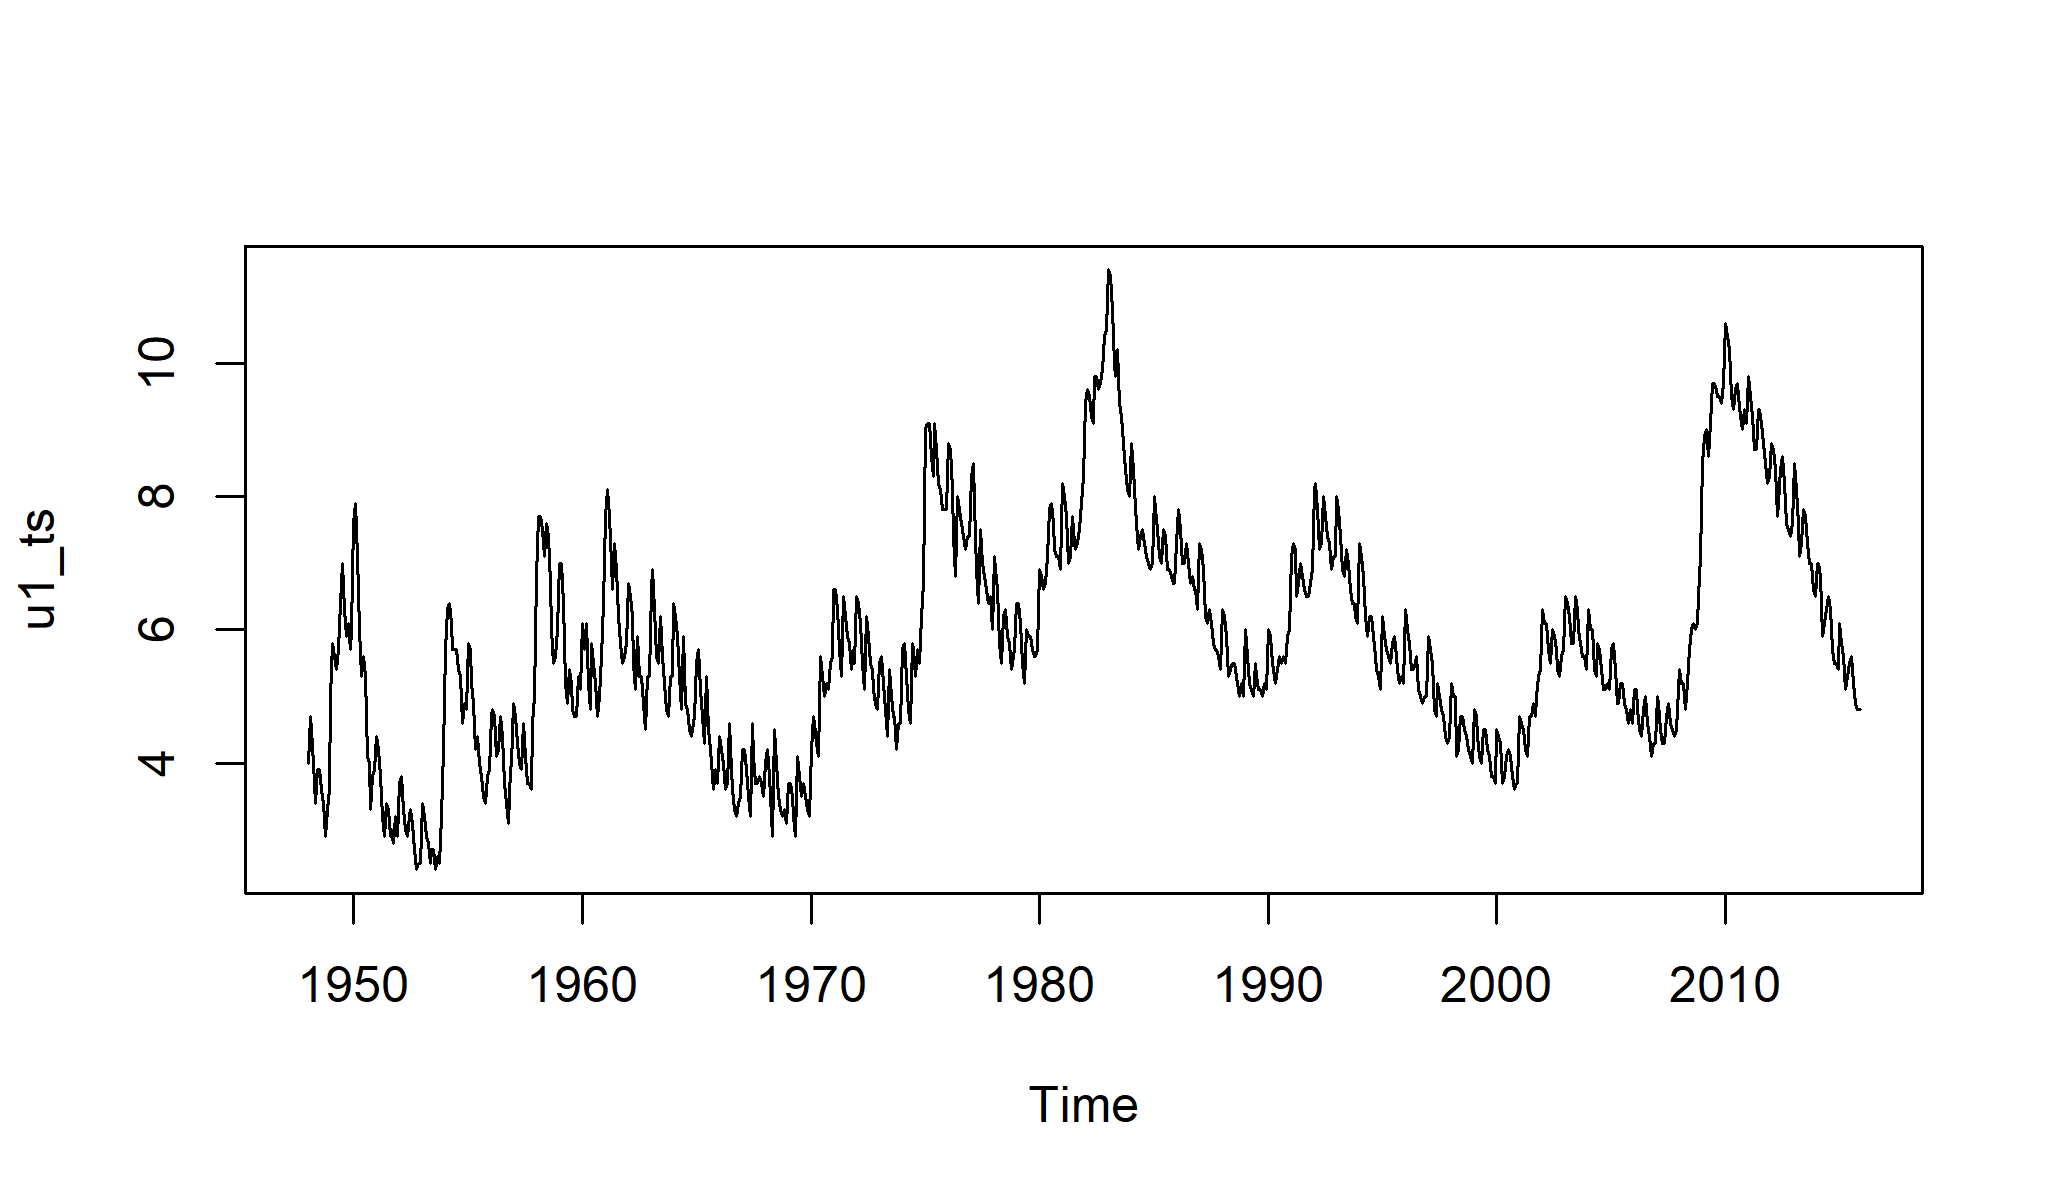
\includegraphics{figure/intro-plot.ts-1} \end{center}

\begin{itemize}
\tightlist
\item
  Note: For a report, we should add units to plots. Also, extra details
  (like \texttt{bandwith} in the periodogram plot) should be explained
  or removed.
\end{itemize}

\subsection{The transfer function (or frequency response function) of a
smoother}\label{the-transfer-function-or-frequency-response-function-of-a-smoother}

\begin{itemize}
\item
  The \hl{ratio of the periodograms of the smoothed and unsmoothed time
  series is called the \textbf{transfer function} or \textbf{frequency
  response function} of the smoother}.
\item
  We can infer the frequency response of the smoother used by Bureau of
  Labor Statistics to deseasonalize the unemployment data.
\end{itemize}

\begin{Shaded}
\begin{Highlighting}[]
\NormalTok{s <-}\StringTok{ }\KeywordTok{spectrum}\NormalTok{(}\KeywordTok{ts.union}\NormalTok{(u1_ts,u2_ts),}\DataTypeTok{plot=}\OtherTok{FALSE}\NormalTok{)}
\end{Highlighting}
\end{Shaded}

\begin{itemize}
\tightlist
\item
  We need to figure out how to extract the bits we need from \texttt{s}
\end{itemize}

\begin{Shaded}
\begin{Highlighting}[]
\KeywordTok{names}\NormalTok{(s)}
\end{Highlighting}
\end{Shaded}

\begin{verbatim}
##  [1] "freq"      "spec"      "coh"       "phase"     "kernel"   
##  [6] "df"        "bandwidth" "n.used"    "orig.n"    "series"   
## [11] "snames"    "method"    "taper"     "pad"       "detrend"  
## [16] "demean"
\end{verbatim}

\begin{Shaded}
\begin{Highlighting}[]
\KeywordTok{dim}\NormalTok{(s}\OperatorTok{$}\NormalTok{spec)}
\end{Highlighting}
\end{Shaded}

\begin{verbatim}
## [1] 432   2
\end{verbatim}

\begin{Shaded}
\begin{Highlighting}[]
\KeywordTok{plot}\NormalTok{(s}\OperatorTok{$}\NormalTok{freq,s}\OperatorTok{\$}\NormalTok{spec[,}\DecValTok{2}\NormalTok{]}\OperatorTok{/}\NormalTok{s}\OperatorTok{\$}\NormalTok{spec[,}\DecValTok{1}\NormalTok{],}\DataTypeTok{type=}\StringTok{"l"}\NormalTok{,}\DataTypeTok{log=}\StringTok{"y"}\NormalTok{,}
  \DataTypeTok{ylab=}\StringTok{"frequency ratio"}\NormalTok{, }\DataTypeTok{xlab=}\StringTok{"frequency"}\NormalTok{,  }
  \DataTypeTok{main=}\StringTok{"frequency response (dashed lines at 0.9 and 1.1)"}\NormalTok{)}
\KeywordTok{abline}\NormalTok{(}\DataTypeTok{h=}\KeywordTok{c}\NormalTok{(}\FloatTok{0.9}\NormalTok{,}\FloatTok{1.1}\NormalTok{),}\DataTypeTok{lty=}\StringTok{"dashed"}\NormalTok{,}\DataTypeTok{col=}\StringTok{"red"}\NormalTok{)}
\end{Highlighting}
\end{Shaded}

\begin{center}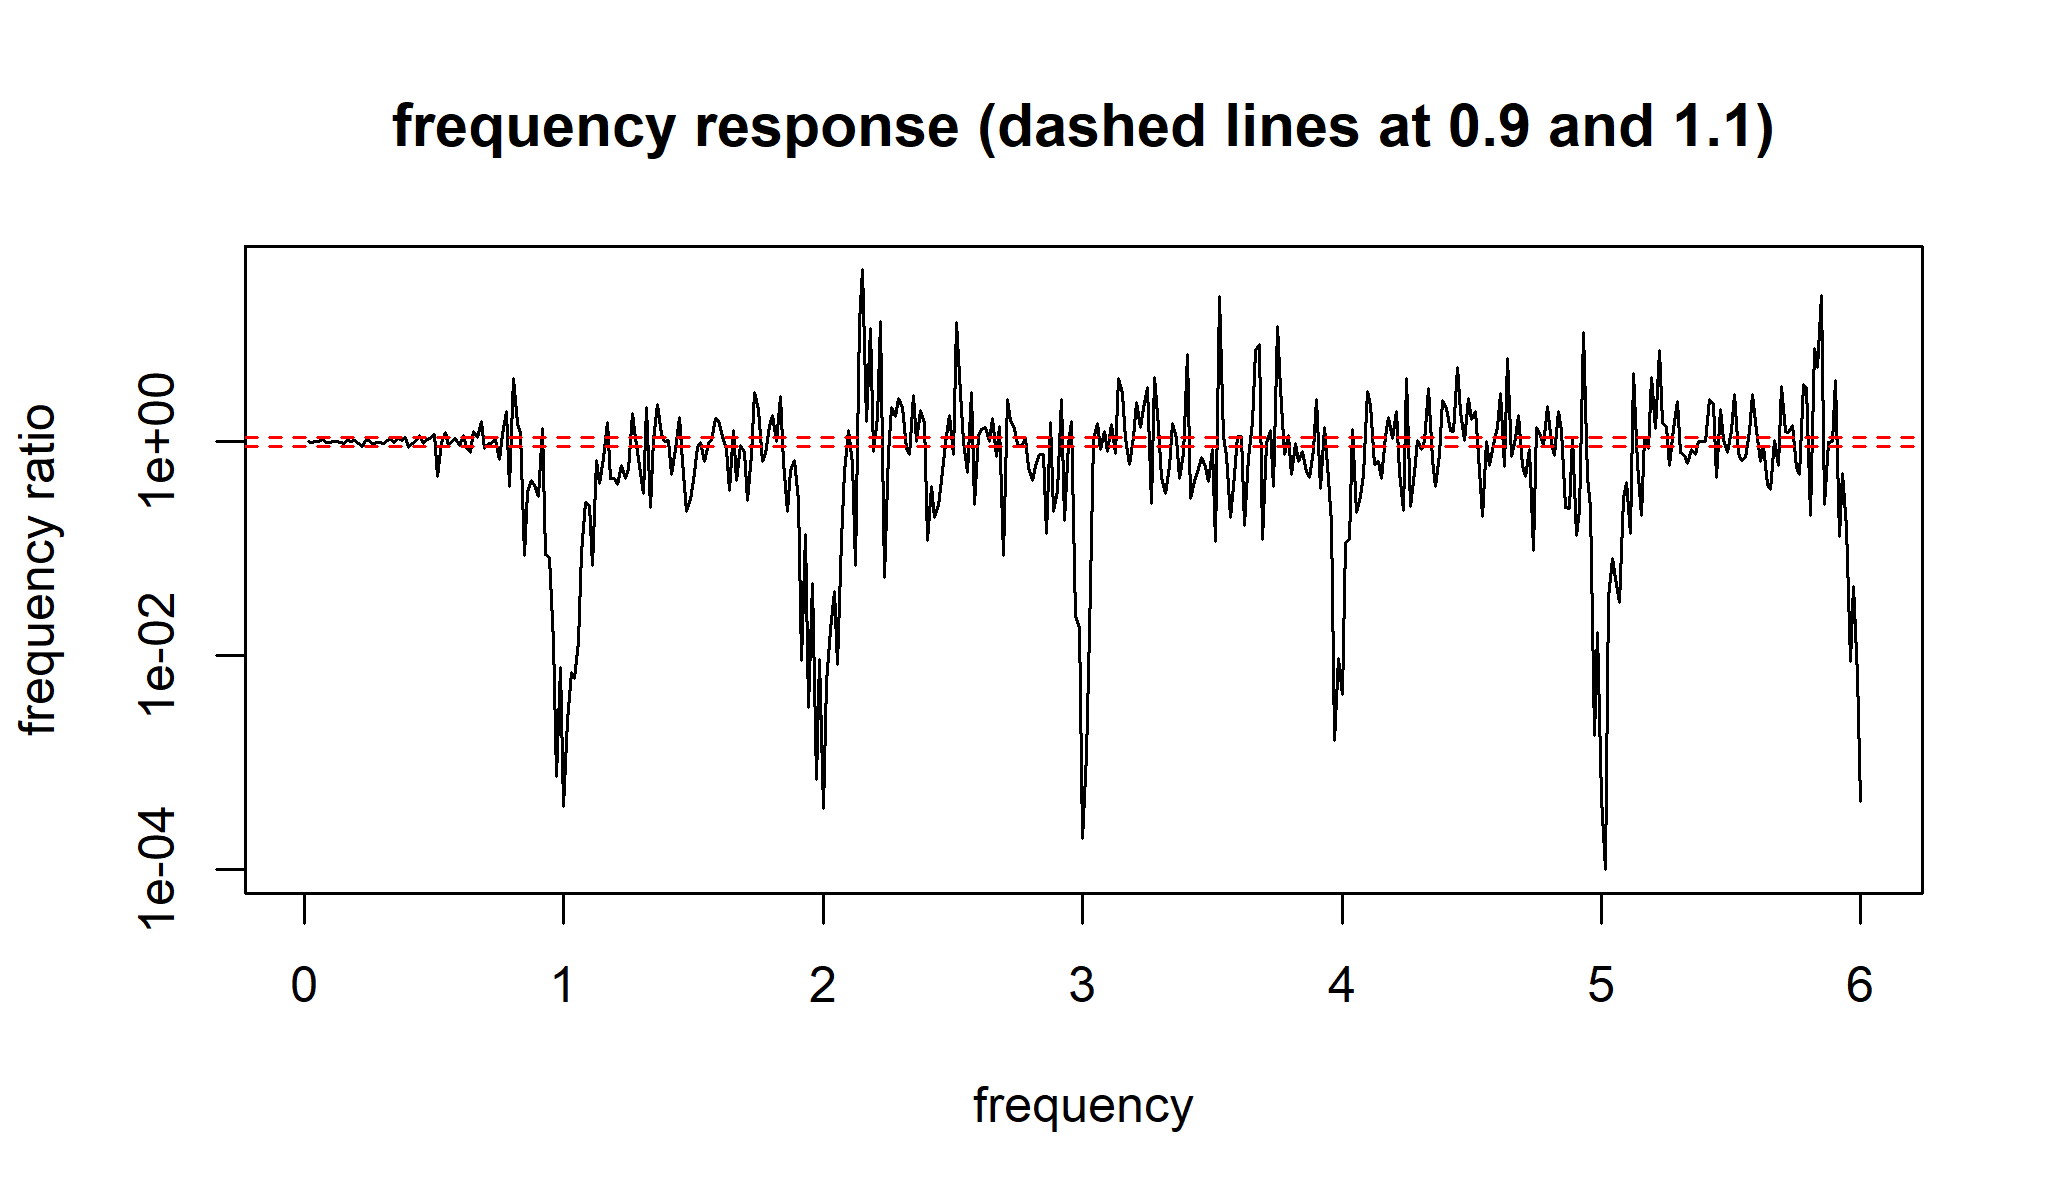
\includegraphics{figure/intro-s_transfer-1} \end{center}

\begin{center}\rule{0.5\linewidth}{\linethickness}\end{center}

\begin{center}\rule{0.5\linewidth}{\linethickness}\end{center}

\subsubsection{Question: What do you learn from this frequency response
plot?}\label{question-what-do-you-learn-from-this-frequency-response-plot}

\begin{center}\rule{0.5\linewidth}{\linethickness}\end{center}

\begin{center}\rule{0.5\linewidth}{\linethickness}\end{center}

\subsubsection{Loess smoothing}\label{loess-smoothing}

\begin{itemize}
\item
  \hl{Loess is a \textbf{Local linear regression} approach} (perhaps an
  acronym for LOcal Estimation by Smoothing?)
\item
  The basic idea is quite simple: at each point in time, we carry out a
  linear regression (e.g., fit a constant, linear or quadratic
  polynomial) using only points close in time. Thus, we can imagine a
  moving window of points included in the regression.
\item
  \texttt{loess} is an R implementation, with the fraction of points
  included in the moving window being scaled by the \texttt{span}
  argument.
\item
  Let's choose a value of the span that visually separates long term
  trend from business cycle.
\end{itemize}

\begin{Shaded}
\begin{Highlighting}[]
\NormalTok{u1_loess <-}\StringTok{ }\KeywordTok{loess}\NormalTok{(u1}\OperatorTok{~}\NormalTok{date,}\DataTypeTok{span=}\FloatTok{0.5}\NormalTok{)}
\KeywordTok{plot}\NormalTok{(date,u1,}\DataTypeTok{type=}\StringTok{"l"}\NormalTok{,}\DataTypeTok{col=}\StringTok{"red"}\NormalTok{)}
\KeywordTok{lines}\NormalTok{(u1_loess}\OperatorTok{\$}\NormalTok{x,u1_loess}\OperatorTok{\$}\NormalTok{fitted,}\DataTypeTok{type=}\StringTok{"l"}\NormalTok{)}
\end{Highlighting}
\end{Shaded}

\begin{center}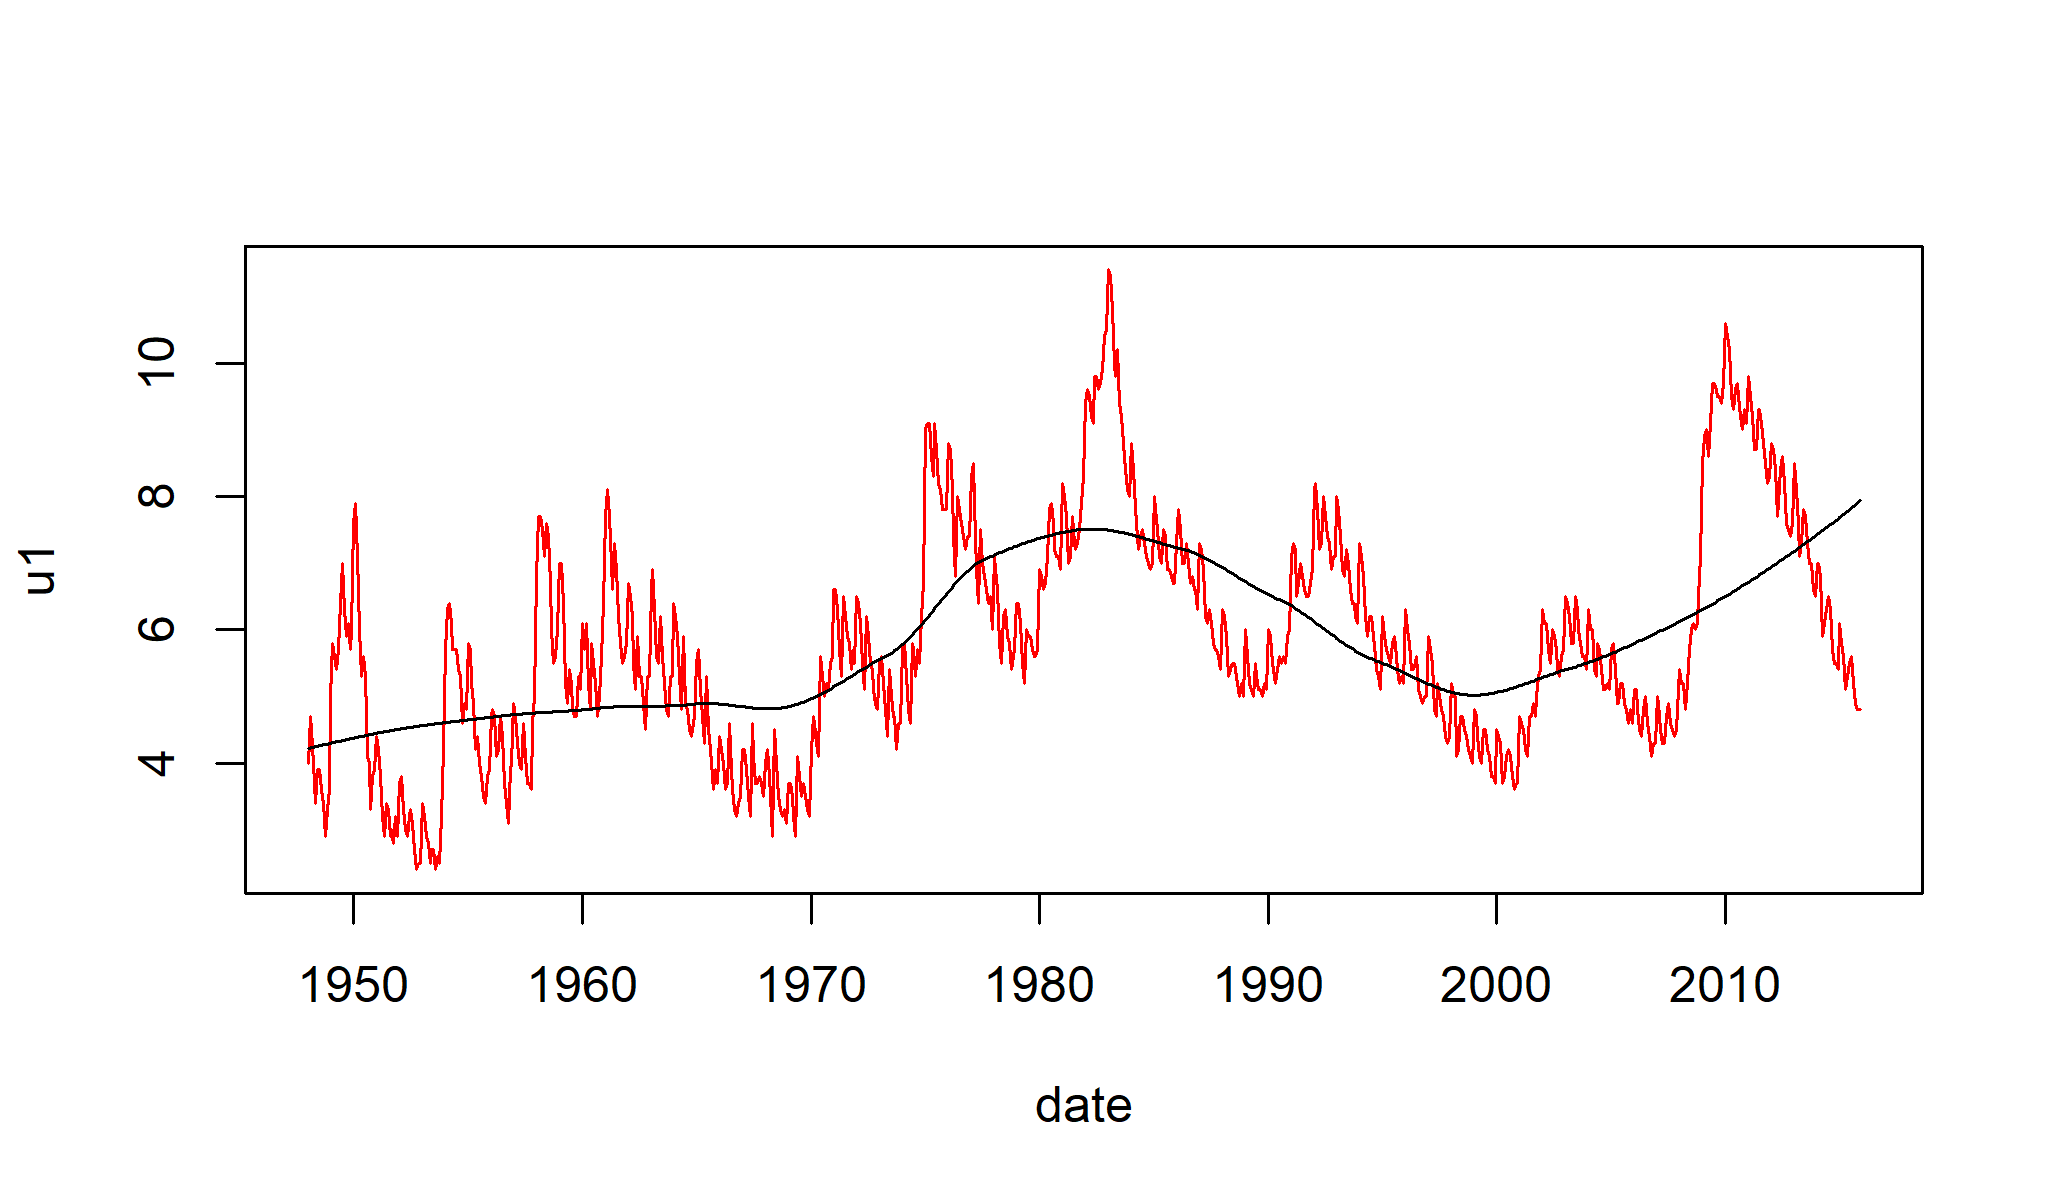
\includegraphics{figure/intro-loess-1} \end{center}

\begin{itemize}
\tightlist
\item
  Now, we can compute the frequency response function for what we have
  done.
\end{itemize}

\begin{Shaded}
\begin{Highlighting}[]
\NormalTok{s2 <-}\StringTok{ }\KeywordTok{spectrum}\NormalTok{(}\KeywordTok{ts.union}\NormalTok{(}
\NormalTok{  u1_ts,}\KeywordTok{ts}\NormalTok{(u1_loess}\OperatorTok{\$}\NormalTok{fitted,}\DataTypeTok{start=}\DecValTok{1948}\NormalTok{,}\DataTypeTok{frequency=}\DecValTok{12}\NormalTok{)),}
  \DataTypeTok{plot=}\OtherTok{FALSE}\NormalTok{)}
\KeywordTok{plot}\NormalTok{(s2}\OperatorTok{\$}\NormalTok{freq,s2}\OperatorTok{\$}\NormalTok{spec[,}\DecValTok{2}\NormalTok{]}\OperatorTok{/}\NormalTok{s}\OperatorTok{\$}\NormalTok{spec[,}\DecValTok{1}\NormalTok{],}\DataTypeTok{type=}\StringTok{"l"}\NormalTok{,}\DataTypeTok{log=}\StringTok{"y"}\NormalTok{,}
  \DataTypeTok{ylab=}\StringTok{"frequency ratio"}\NormalTok{, }\DataTypeTok{xlab=}\StringTok{"frequency"}\NormalTok{, }\DataTypeTok{xlim=}\KeywordTok{c}\NormalTok{(}\DecValTok{0}\NormalTok{,}\FloatTok{1.5}\NormalTok{),}
  \DataTypeTok{main=}\StringTok{"frequency response (dashed line at 1.0)"}\NormalTok{)}
\KeywordTok{abline}\NormalTok{(}\DataTypeTok{h=}\DecValTok{1}\NormalTok{,}\DataTypeTok{lty=}\StringTok{"dashed"}\NormalTok{,}\DataTypeTok{col=}\StringTok{"red"}\NormalTok{)}
\end{Highlighting}
\end{Shaded}

\begin{center}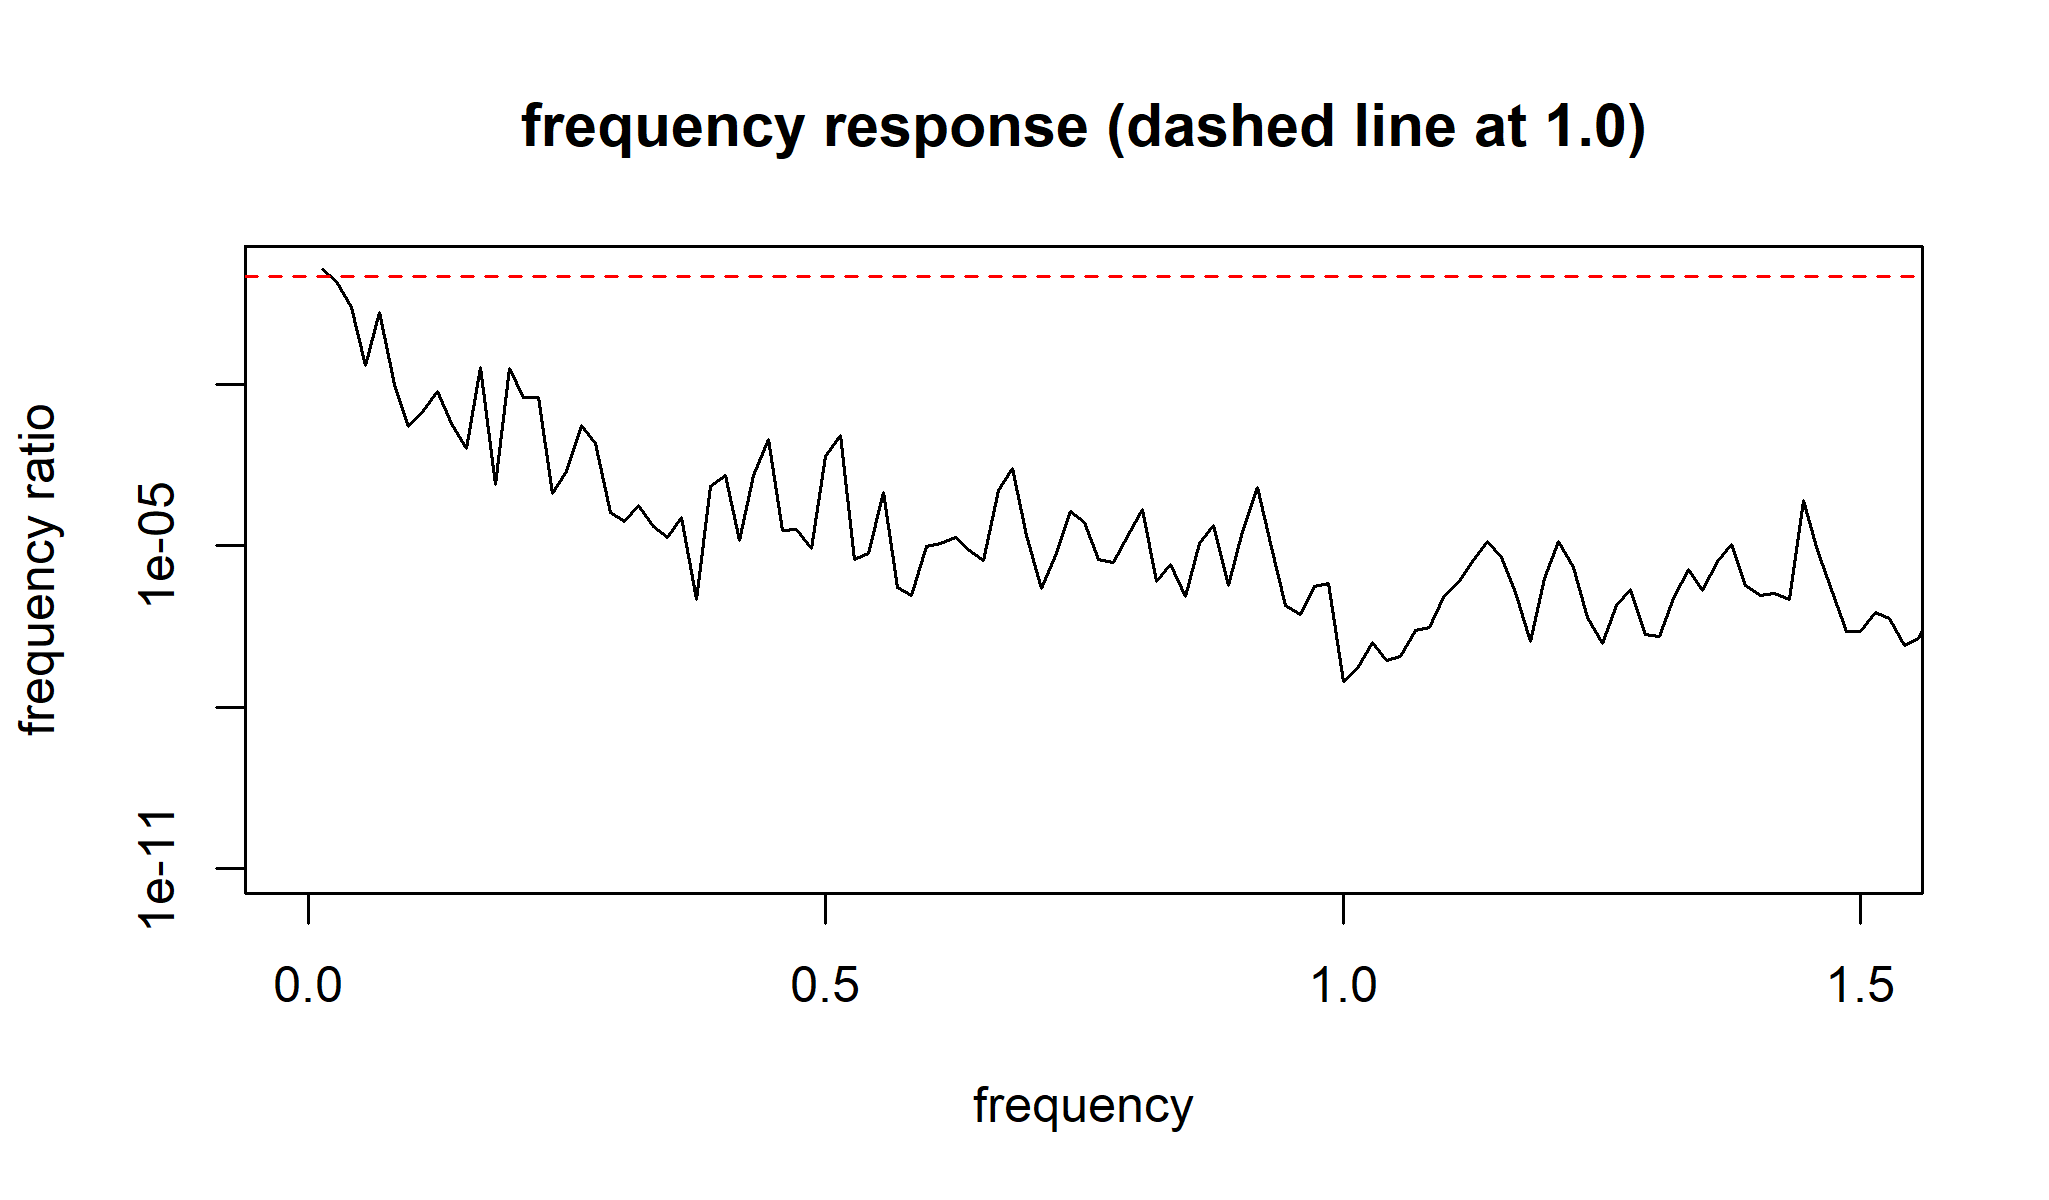
\includegraphics{figure/intro-loess_transfer-1} \end{center}

\begin{center}\rule{0.5\linewidth}{\linethickness}\end{center}

\begin{center}\rule{0.5\linewidth}{\linethickness}\end{center}

\subsubsection{Question: Describe the frequency domain behavior of this
filter.}\label{question-describe-the-frequency-domain-behavior-of-this-filter.}

\begin{center}\rule{0.5\linewidth}{\linethickness}\end{center}

\begin{center}\rule{0.5\linewidth}{\linethickness}\end{center}

\subsection{Extracting business cycles: A band pass
filter}\label{extracting-business-cycles-a-band-pass-filter}

\begin{itemize}
\item
  For the unemployment data, high frequency variation might be
  considered ``noise'' and low frequency variation might be considered
  trend.
\item
  A band of mid-range frequencies might be considered to correspond to
  the business cycle.
\item
  Let's build a smoothing operation in the time domain to extract
  business cycles, and then look at its frequency response function.
\end{itemize}

\begin{Shaded}
\begin{Highlighting}[]
\NormalTok{u_low <-}\StringTok{ }\KeywordTok{ts}\NormalTok{(}\KeywordTok{loess}\NormalTok{(u1}\OperatorTok{~}\NormalTok{date,}\DataTypeTok{span=}\FloatTok{0.5}\NormalTok{)}\OperatorTok{\$}\NormalTok{fitted,}\DataTypeTok{start=}\DecValTok{1948}\NormalTok{,}\DataTypeTok{frequency=}\DecValTok{12}\NormalTok{)}
\NormalTok{u_hi <-}\StringTok{ }\KeywordTok{ts}\NormalTok{(u1 }\OperatorTok{-}\StringTok{ }\KeywordTok{loess}\NormalTok{(u1}\OperatorTok{~}\NormalTok{date,}\DataTypeTok{span=}\FloatTok{0.1}\NormalTok{)}\OperatorTok{\$}\NormalTok{fitted,}\DataTypeTok{start=}\DecValTok{1948}\NormalTok{,}\DataTypeTok{frequency=}\DecValTok{12}\NormalTok{)}
\NormalTok{u_cycles <-}\StringTok{ }\NormalTok{u1 }\OperatorTok{-}\StringTok{ }\NormalTok{u_hi }\OperatorTok{-}\StringTok{ }\NormalTok{u_low}
\KeywordTok{plot}\NormalTok{(}\KeywordTok{ts.union}\NormalTok{(u1, u_low,u_hi,u_cycles),}
  \DataTypeTok{main=}\StringTok{"Decomposition of unemployment as trend + noise + cycles"}\NormalTok{)}
\end{Highlighting}
\end{Shaded}

\begin{center}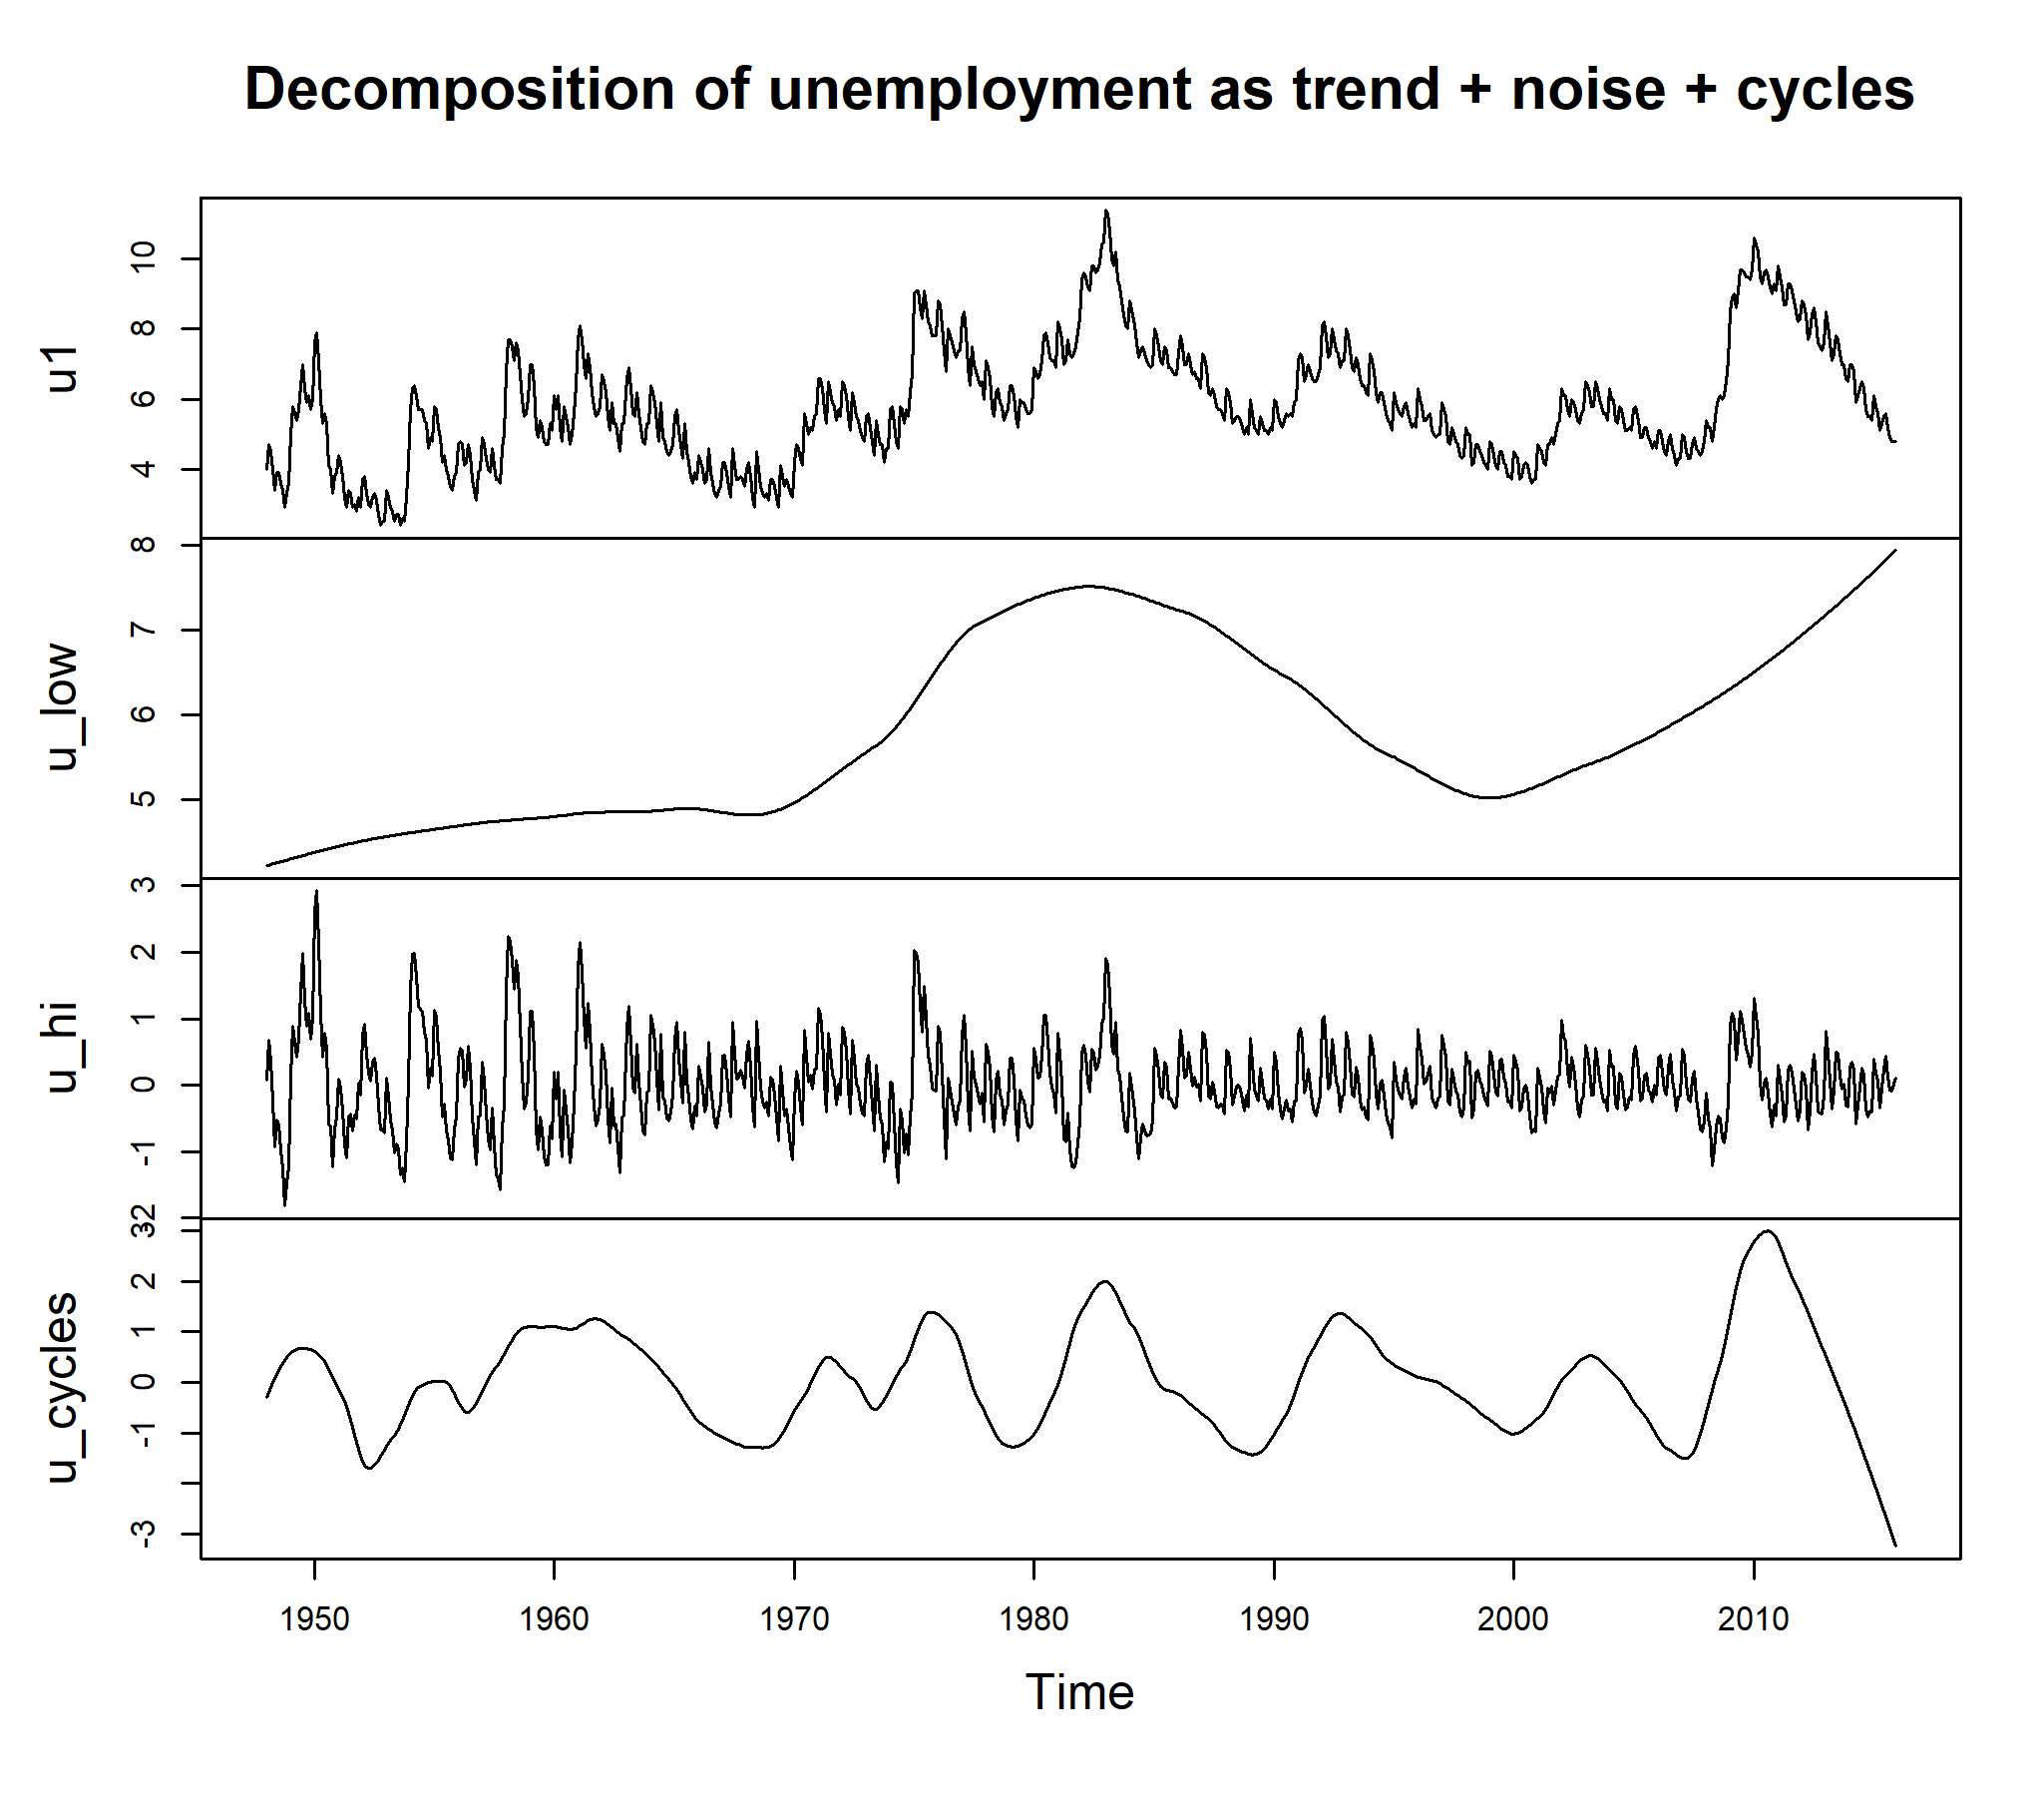
\includegraphics{figure/intro-cycles-1} \end{center}

\begin{Shaded}
\begin{Highlighting}[]
\NormalTok{spec_cycle <-}\StringTok{ }\KeywordTok{spectrum}\NormalTok{(}\KeywordTok{ts.union}\NormalTok{(u1_ts,u_cycles),}
  \DataTypeTok{spans=}\KeywordTok{c}\NormalTok{(}\DecValTok{3}\NormalTok{,}\DecValTok{3}\NormalTok{),}
  \DataTypeTok{plot=}\OtherTok{FALSE}\NormalTok{)}
\NormalTok{freq_response_cycle <-}\StringTok{ }\NormalTok{spec_cycle}\OperatorTok{\$}\NormalTok{spec[,}\DecValTok{2}\NormalTok{]}\OperatorTok{/}\NormalTok{spec_cycle}\OperatorTok{\$}\NormalTok{spec[,}\DecValTok{1}\NormalTok{]}
\KeywordTok{plot}\NormalTok{(spec_cycle}\OperatorTok{\$}\NormalTok{freq,freq_response_cycle,}
  \DataTypeTok{type=}\StringTok{"l"}\NormalTok{,}\DataTypeTok{log=}\StringTok{"y"}\NormalTok{,}
  \DataTypeTok{ylab=}\StringTok{"frequency ratio"}\NormalTok{, }\DataTypeTok{xlab=}\StringTok{"frequency"}\NormalTok{, }\DataTypeTok{xlim=}\KeywordTok{c}\NormalTok{(}\DecValTok{0}\NormalTok{,}\FloatTok{1.2}\NormalTok{), }\DataTypeTok{ylim=}\KeywordTok{c}\NormalTok{(}\FloatTok{5e-6}\NormalTok{,}\FloatTok{1.1}\NormalTok{),}
  \DataTypeTok{main=}\StringTok{"frequency response (dashed line at 1.0)"}\NormalTok{)}
\KeywordTok{abline}\NormalTok{(}\DataTypeTok{h=}\DecValTok{1}\NormalTok{,}\DataTypeTok{lty=}\StringTok{"dashed"}\NormalTok{,}\DataTypeTok{col=}\StringTok{"red"}\NormalTok{)  }
\end{Highlighting}
\end{Shaded}

\begin{center}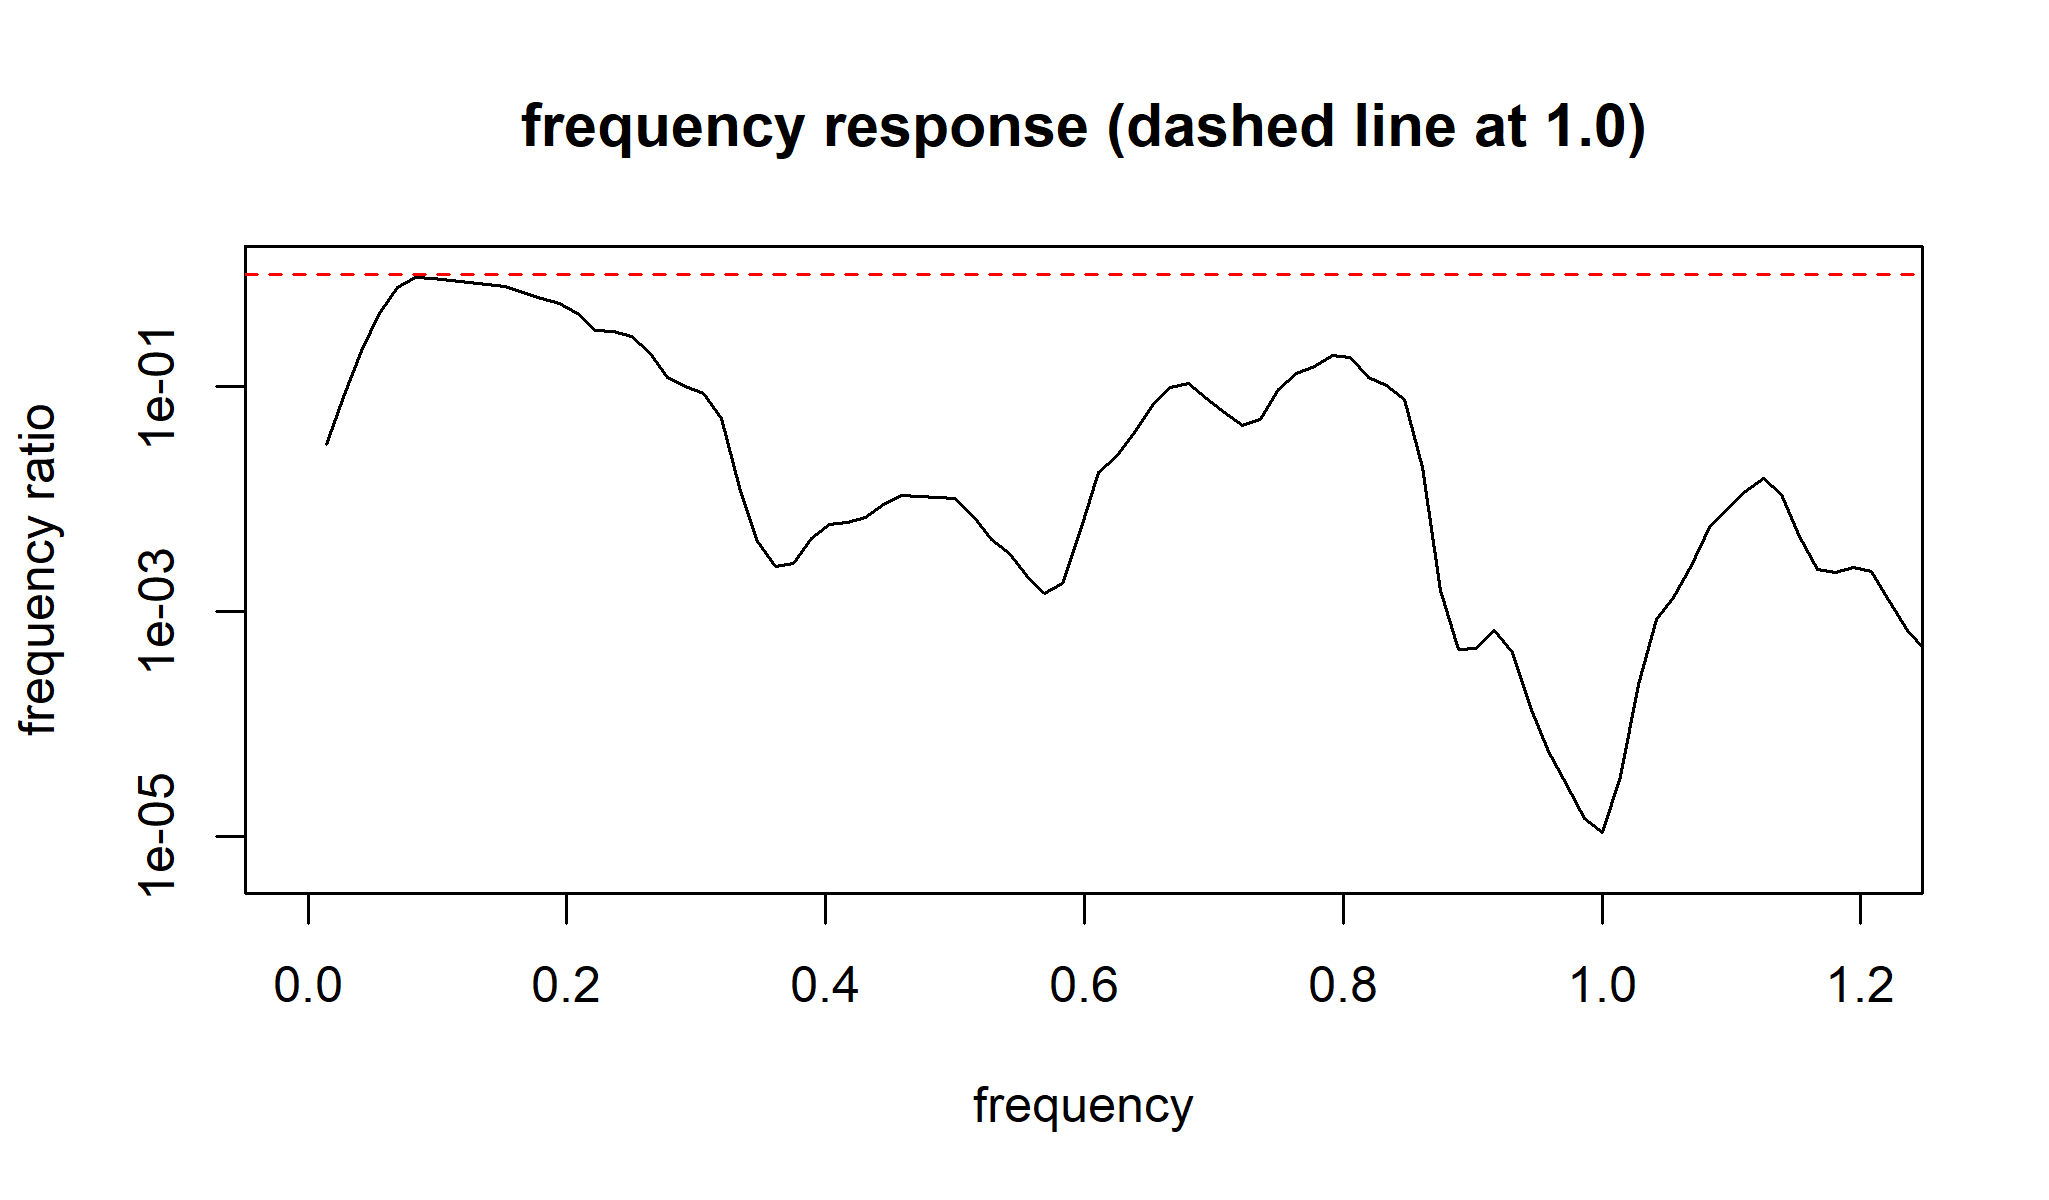
\includegraphics{figure/intro-freq_response-1} \end{center}

\begin{center}\rule{0.5\linewidth}{\linethickness}\end{center}

\begin{center}\rule{0.5\linewidth}{\linethickness}\end{center}

\subsubsection{Question: Describe the frequencies (and corresponding
periods) that this decomposition identifies as business
cycles}\label{question-describe-the-frequencies-and-corresponding-periods-that-this-decomposition-identifies-as-business-cycles}

\begin{itemize}
\item
  Note: Usually, we should specify units for frequency and period. Here,
  the units are omitted to give you an exercise!
\item
  To help answer this question, let's add some lines to the previous
  plot
\end{itemize}

\begin{Shaded}
\begin{Highlighting}[]
\NormalTok{cut_fraction <-}\StringTok{ }\FloatTok{0.5}
\KeywordTok{plot}\NormalTok{(spec_cycle}\OperatorTok{\$}\NormalTok{freq,freq_response_cycle,}
  \DataTypeTok{type=}\StringTok{"l"}\NormalTok{,}\DataTypeTok{log=}\StringTok{"y"}\NormalTok{,}
  \DataTypeTok{ylab=}\StringTok{"frequency ratio"}\NormalTok{, }\DataTypeTok{xlab=}\StringTok{"frequency"}\NormalTok{, }\DataTypeTok{xlim=}\KeywordTok{c}\NormalTok{(}\DecValTok{0}\NormalTok{,}\FloatTok{0.9}\NormalTok{), }\DataTypeTok{ylim=}\KeywordTok{c}\NormalTok{(}\FloatTok{1e-4}\NormalTok{,}\FloatTok{1.1}\NormalTok{),}
  \DataTypeTok{main=}\KeywordTok{paste}\NormalTok{(}\StringTok{"frequency response, showing region for ratio >"}\NormalTok{, cut_fraction))}
\KeywordTok{abline}\NormalTok{(}\DataTypeTok{h=}\DecValTok{1}\NormalTok{,}\DataTypeTok{lty=}\StringTok{"dashed"}\NormalTok{,}\DataTypeTok{col=}\StringTok{"blue"}\NormalTok{)  }
\NormalTok{freq_cycles <-}\StringTok{ }\KeywordTok{range}\NormalTok{(spec_cycle}\OperatorTok{\$}\NormalTok{freq[freq_response_cycle}\OperatorTok{>}\NormalTok{cut_fraction]) }
\KeywordTok{abline}\NormalTok{(}\DataTypeTok{v=}\NormalTok{freq_cycles,}\DataTypeTok{lty=}\StringTok{"dashed"}\NormalTok{,}\DataTypeTok{col=}\StringTok{"blue"}\NormalTok{) }
\KeywordTok{abline}\NormalTok{(}\DataTypeTok{h=}\NormalTok{cut_fraction,}\DataTypeTok{lty=}\StringTok{"dashed"}\NormalTok{,}\DataTypeTok{col=}\StringTok{"blue"}\NormalTok{)}
\end{Highlighting}
\end{Shaded}

\begin{center}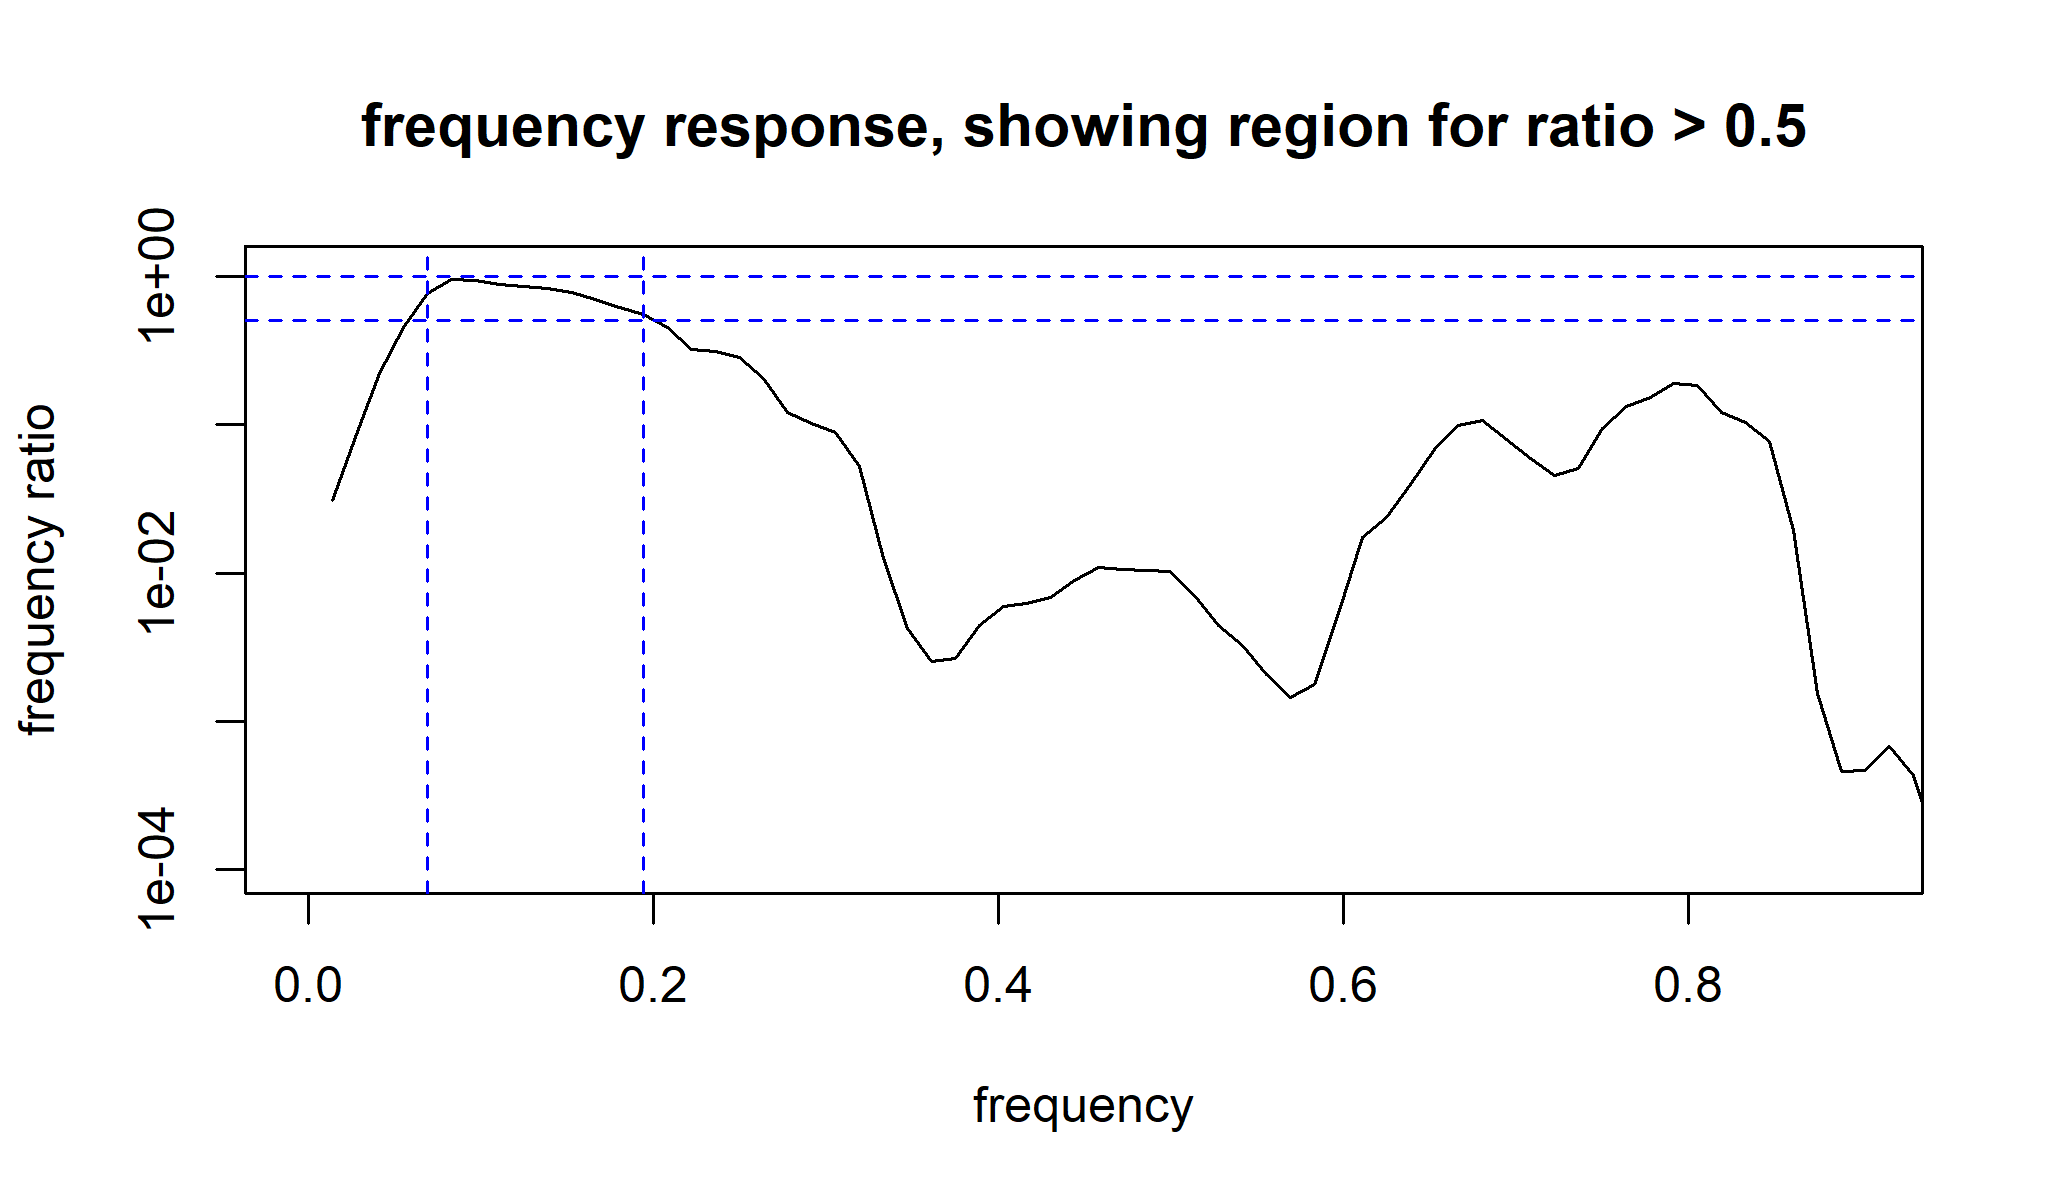
\includegraphics{figure/intro-show_range-1} \end{center}

\begin{Shaded}
\begin{Highlighting}[]
\KeywordTok{kable}\NormalTok{(}\KeywordTok{matrix}\NormalTok{(freq_cycles,}\DataTypeTok{nrow=}\DecValTok{1}\NormalTok{,}\DataTypeTok{dimnames=}\KeywordTok{list}\NormalTok{(}\StringTok{"frequency"}\NormalTok{,}\KeywordTok{c}\NormalTok{(}\StringTok{"low"}\NormalTok{,}\StringTok{"hi"}\NormalTok{))),}\DataTypeTok{digits=}\DecValTok{3}\NormalTok{)}
\end{Highlighting}
\end{Shaded}

\begin{longtable}[]{@{}lrr@{}}
\toprule
& low & hi\tabularnewline
\midrule
\endhead
frequency & 0.069 & 0.194\tabularnewline
\bottomrule
\end{longtable}

\begin{center}\rule{0.5\linewidth}{\linethickness}\end{center}

\begin{center}\rule{0.5\linewidth}{\linethickness}\end{center}

\subsubsection{Question: So far as we have opinions on business cycles,
use them to criticize this
decomposition.}\label{question-so-far-as-we-have-opinions-on-business-cycles-use-them-to-criticize-this-decomposition.}

\begin{center}\rule{0.5\linewidth}{\linethickness}\end{center}

\begin{center}\rule{0.5\linewidth}{\linethickness}\end{center}

\subsubsection{Question: Criticizing the construction of the blue dashed
lines}\label{question-criticizing-the-construction-of-the-blue-dashed-lines}

\begin{itemize}
\item
  Why do the blue dashed lines in the above figure not meet exactly on
  the frequency response curve?
\item
  What could or should be done to improve this?
\end{itemize}

\begin{center}\rule{0.5\linewidth}{\linethickness}\end{center}

\begin{center}\rule{0.5\linewidth}{\linethickness}\end{center}

\subsubsection{Looking for business
cycles}\label{looking-for-business-cycles}

\begin{itemize}
\item
  We can plot just the lower frequencies of a smoothed periodogram for
  the raw unemployment data, to zoom in on the frequencies around the
  business cycle frequency.
\item
  Standard periodogram smoothers use the same smoothing bandwidth across
  all frequencies. This may not always be appropriate. Why?
\item
  Sometimes in practice we want to use less smoothing when we are
  focusing on low frequency behaviors.
\end{itemize}

\begin{Shaded}
\begin{Highlighting}[]
\NormalTok{s1 <-}\StringTok{ }\KeywordTok{spectrum}\NormalTok{(u1_ts,}\DataTypeTok{spans=}\KeywordTok{c}\NormalTok{(}\DecValTok{3}\NormalTok{),}\DataTypeTok{plot=}\OtherTok{FALSE}\NormalTok{)}
\KeywordTok{plot}\NormalTok{(s1,}\DataTypeTok{xlim=}\KeywordTok{c}\NormalTok{(}\DecValTok{0}\NormalTok{,}\FloatTok{0.7}\NormalTok{),}\DataTypeTok{ylim=}\KeywordTok{c}\NormalTok{(}\FloatTok{1e-2}\NormalTok{,}\KeywordTok{max}\NormalTok{(s1}\OperatorTok{\$}\NormalTok{spec)))}
\end{Highlighting}
\end{Shaded}

\begin{center}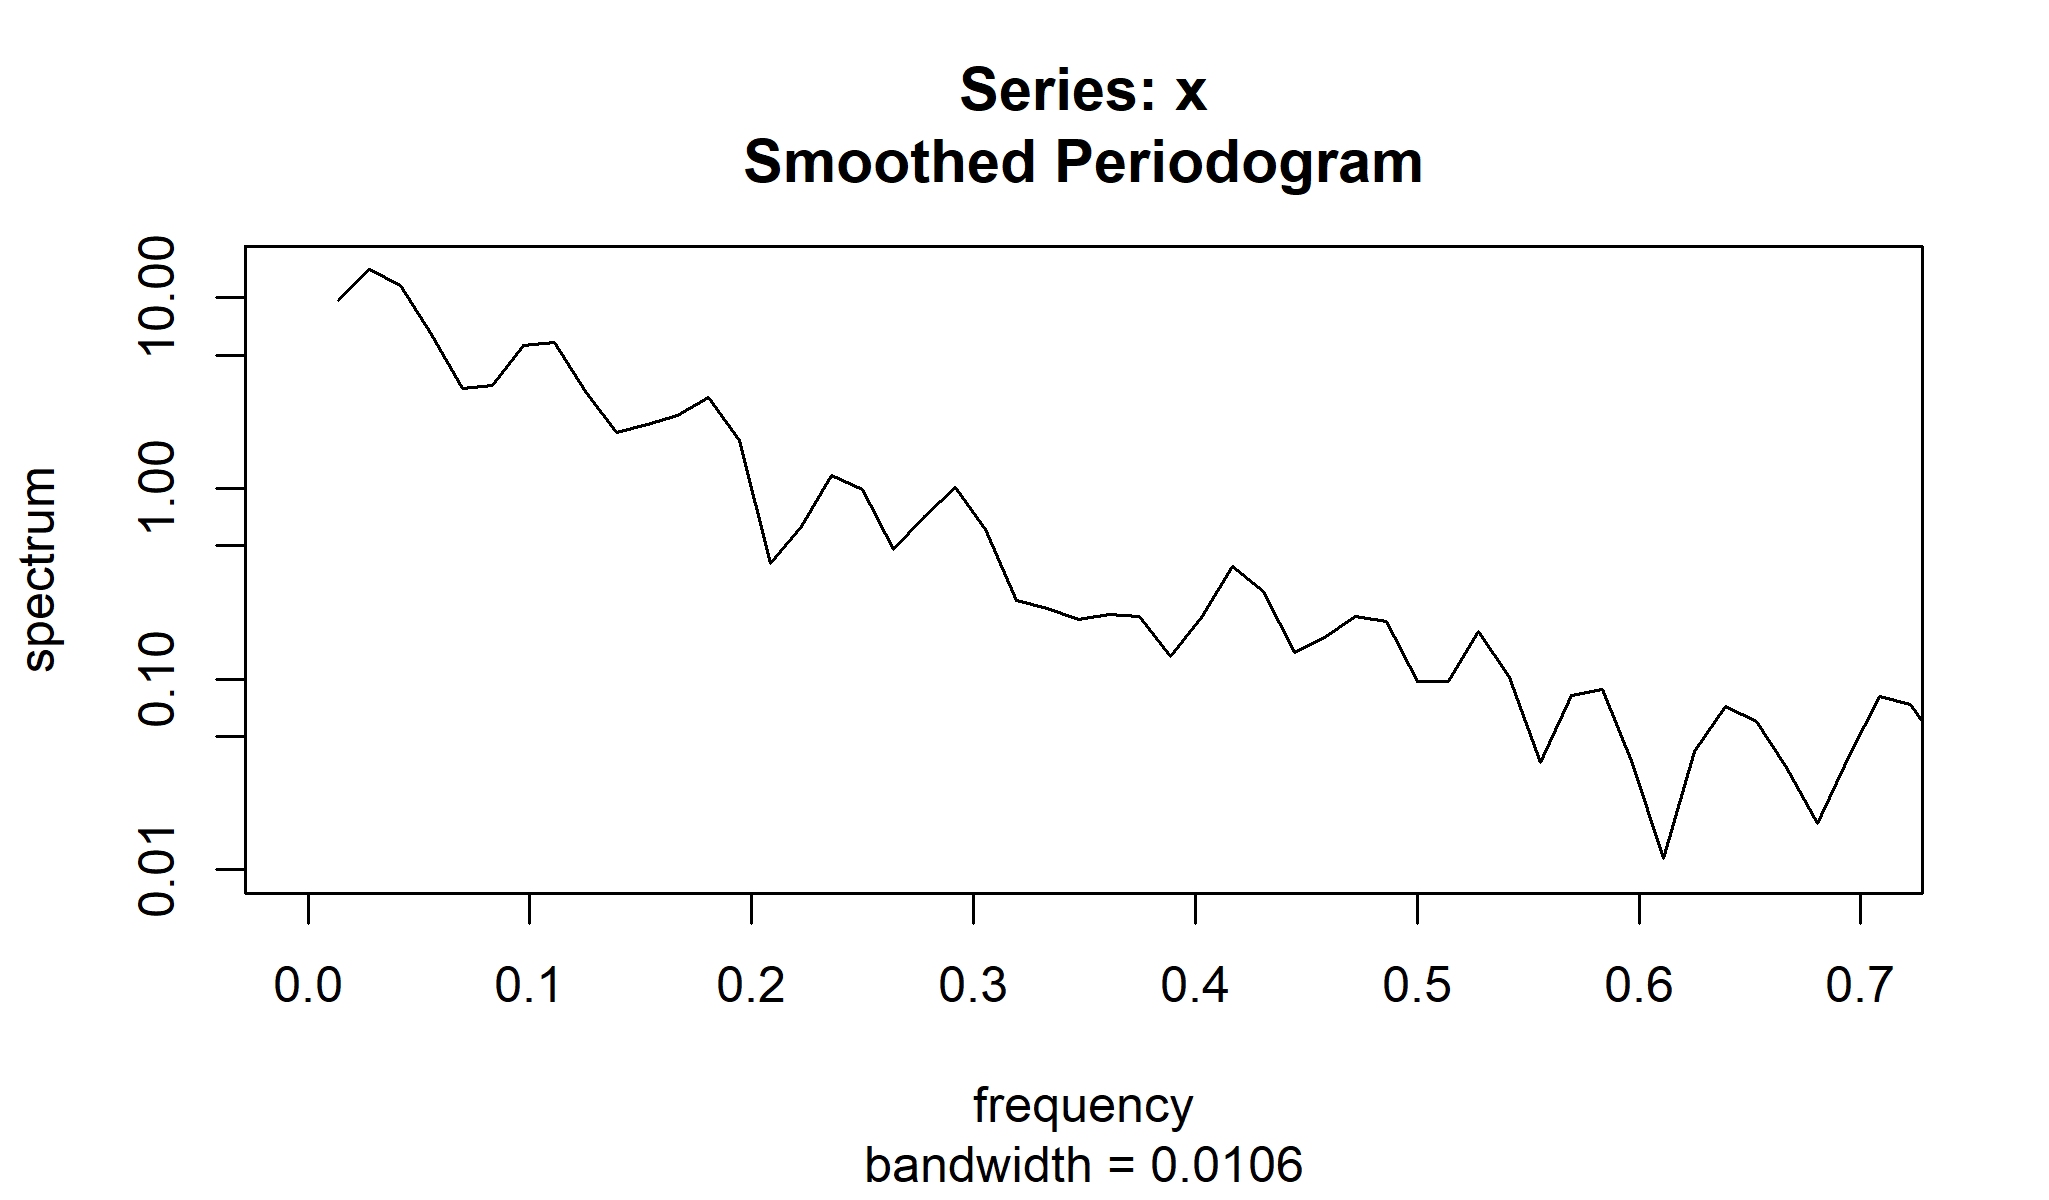
\includegraphics{figure/intro-zoomed_spectrum-1} \end{center}

\begin{center}\rule{0.5\linewidth}{\linethickness}\end{center}

\begin{center}\rule{0.5\linewidth}{\linethickness}\end{center}

\subsubsection{Question: Comment on the evidence for and against the
concept of a business cycle in the above
figure.}\label{question-comment-on-the-evidence-for-and-against-the-concept-of-a-business-cycle-in-the-above-figure.}

\begin{center}\rule{0.5\linewidth}{\linethickness}\end{center}

\begin{center}\rule{0.5\linewidth}{\linethickness}\end{center}

\subsection{Common smoothers in R}\label{common-smoothers-in-r}

\begin{itemize}
\item
  Above, we have used the \textbf{local regression smoother}
  \texttt{loess} but there are other options.
\item
  Our immediate goal is to get practical experience using a smoother and
  then statistically assessing what we have done.
\item
  You can learn about alternative smoothers, and try them out, if you
  like.
\item
  \texttt{ksmooth} is a
  \href{https://en.wikipedia.org/wiki/Kernel_smoother}{\textbf{kernel
  smoother}}. The default periodogram smoother in \texttt{spectrum} is
  also a kernel smoother.
\item
  \texttt{smooth.spline} is a
  \href{https://en.wikipedia.org/wiki/Smoothing_spline}{\textbf{spline
  smoother}}.
\item
  All these smoothers have some concept of a \textbf{bandwidth}, which
  is a measure of the size of the neighborhood of time points in which
  data affect the smoothed value at a particular time point.
\item
  The concept of bandwidth is most obvious for kernel smoothers, but
  exists for other smoothers.
\item
  We usually only interpret bandwidth up to a constant. For a particular
  smoothing algorithm and software implementation, you learn by
  experience to interpret the comparative value (smaller bandwidth means
  less smoothing).
\item
  Typically, when writing reports, it makes sense not to present or
  discuss smoothing bandwidth since it is not directly interpretable for
  most readers.
\end{itemize}

\begin{center}\rule{0.5\linewidth}{\linethickness}\end{center}

\begin{center}\rule{0.5\linewidth}{\linethickness}\end{center}


\end{document}
